\documentclass[10pt,letterpaper]{article}
\usepackage{geometry}
\geometry{legalpaper, portrait, margin=0.2in}
\usepackage[utf8]{inputenc}
\usepackage{amsmath}
\usepackage{amsfonts}
\usepackage{amssymb}
\usepackage{graphicx}
\usepackage{subcaption}
\usepackage{array}
\usepackage{pdfpages}


\pdfobjcompresslevel=0

\begin{document}

CL0034 Target 11, Arm 22 \\

\begin{table}[h!]
\begin{center}
\begin{tabular}{ >{\centering\arraybackslash}m{2.5in} >{\centering\arraybackslash}m{2.5in} >{\centering\arraybackslash}m{2.5in} >{\centering\arraybackslash}m{2.3in} }
HST Image & Collapsed YJ Image &  Collapsed IZ Image & \\
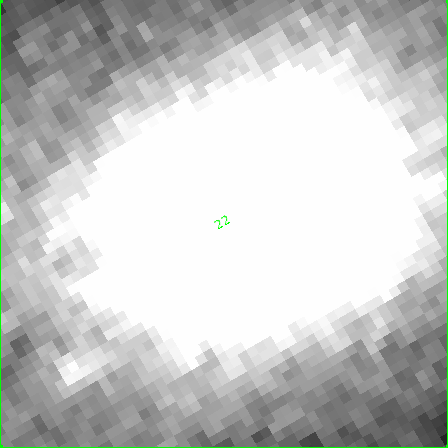
\includegraphics[scale=0.35]{/home/rburnet/S16work/diagnostic_of_objects/figures/HST_images/CL0034/CL0034-Target_11.png} 
& 
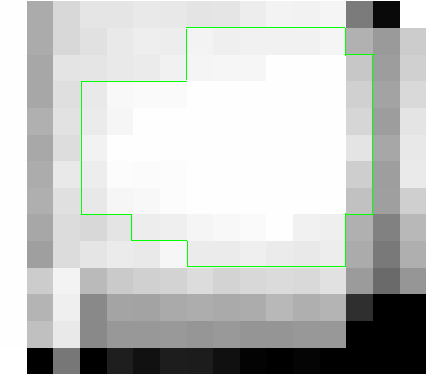
\includegraphics[scale=0.4]{/home/rburnet/S16work/diagnostic_of_objects/local_sky_subtraction/new_report/figures/CL0034-IZ-Target_11.png} 
&
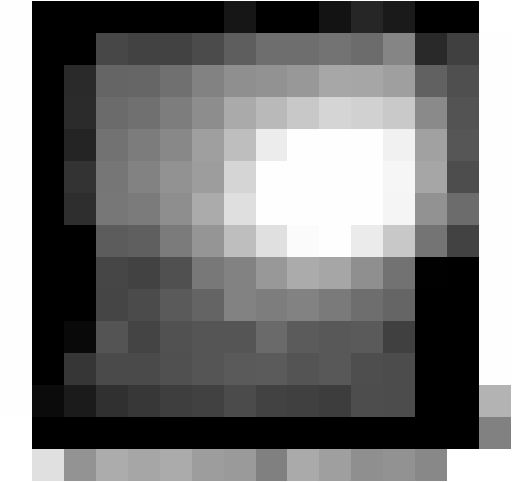
\includegraphics[scale=0.4]{/home/rburnet/S16work/diagnostic_of_objects/local_sky_subtraction/new_report/figures/CL0034-YJ-Target_11.png} 
\\
& 
\begin{tabular}{ l l l }
M$_{\text{IZ, calculated}}$ & = &  19.99\\
M$_{\text{YJ, calculated}}$ & = &  19.55\\
M$_{\text{Z, expected}}$ & = & 19.43\\
F(H$\alpha) _{\text{expected}}$ & = & 2.190e-15\\
F(H$\alpha) _{\text{expected, uncorrected}}$ & = & 6.223e-16\\
\end{tabular} \\
\\
%\begin{tabular}{l}
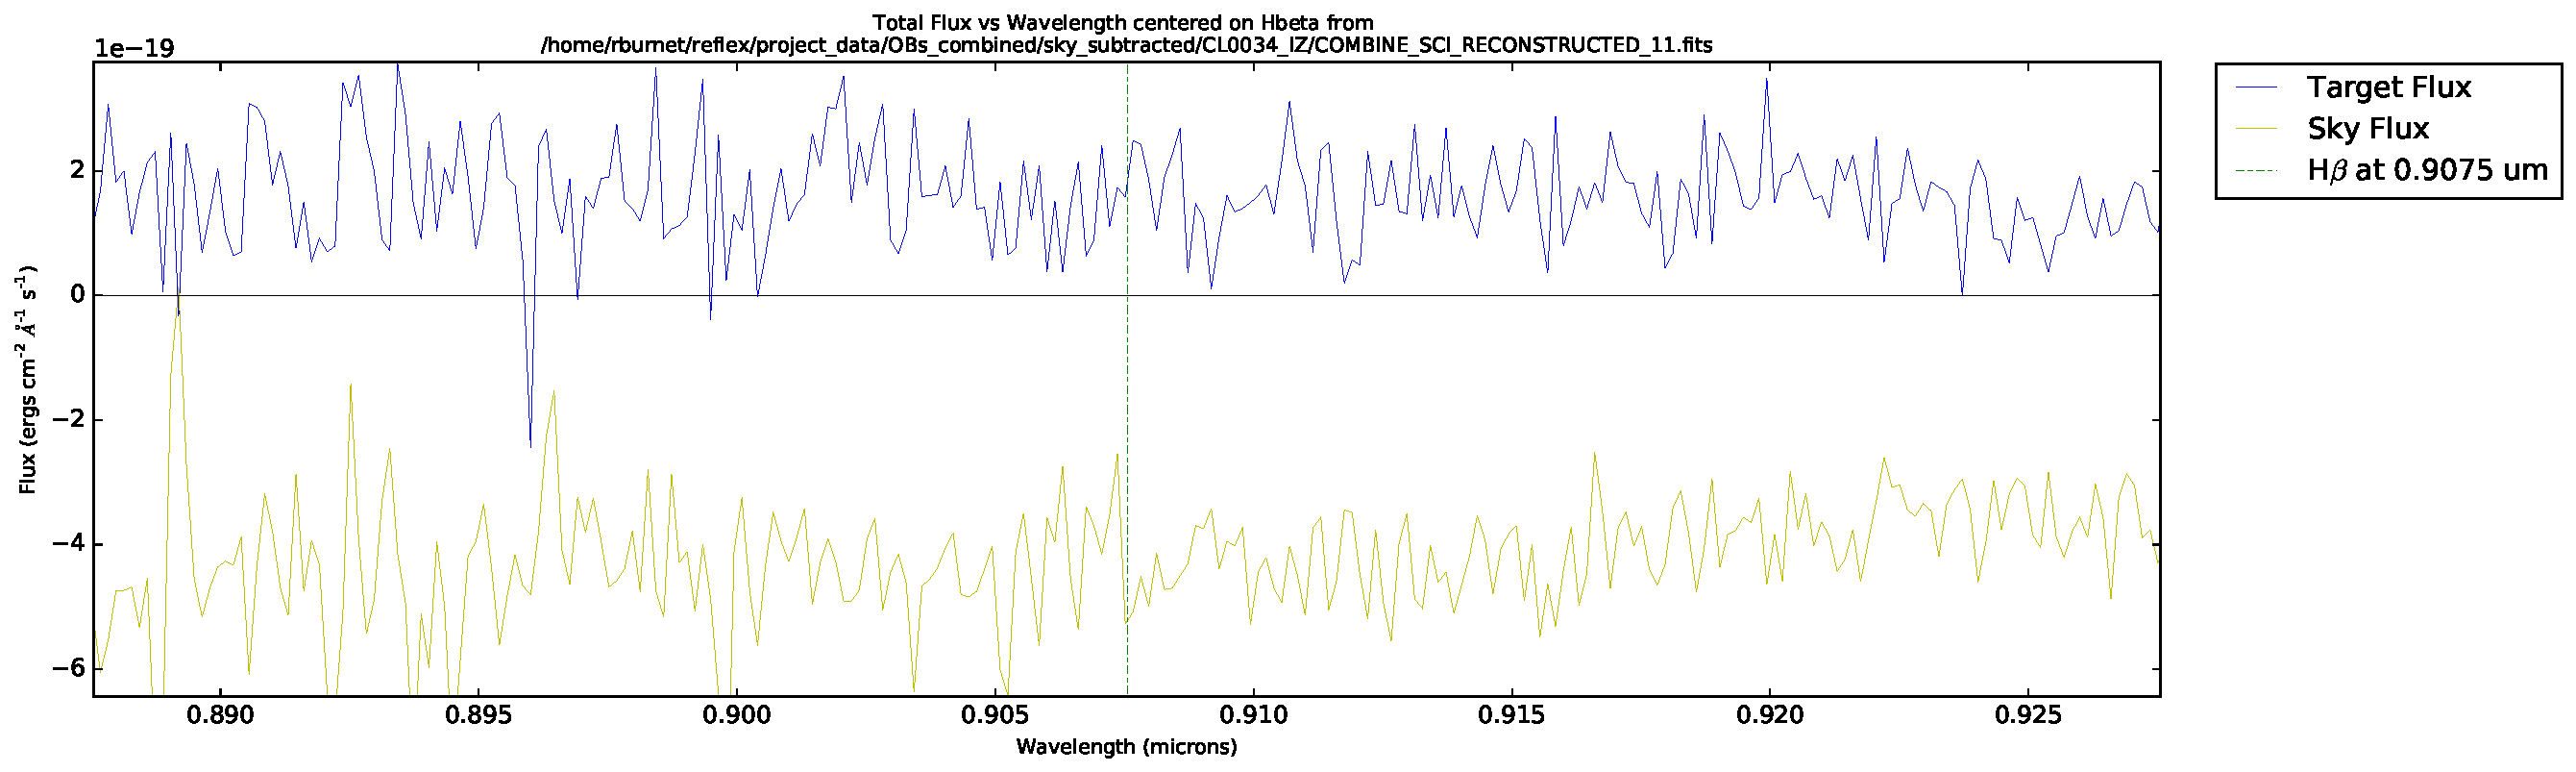
\includegraphics[scale=0.45]{../figures/CL0034_IZ/COMBINE_SCI_RECONSTRUCTED_11_Hbeta.pdf} \\
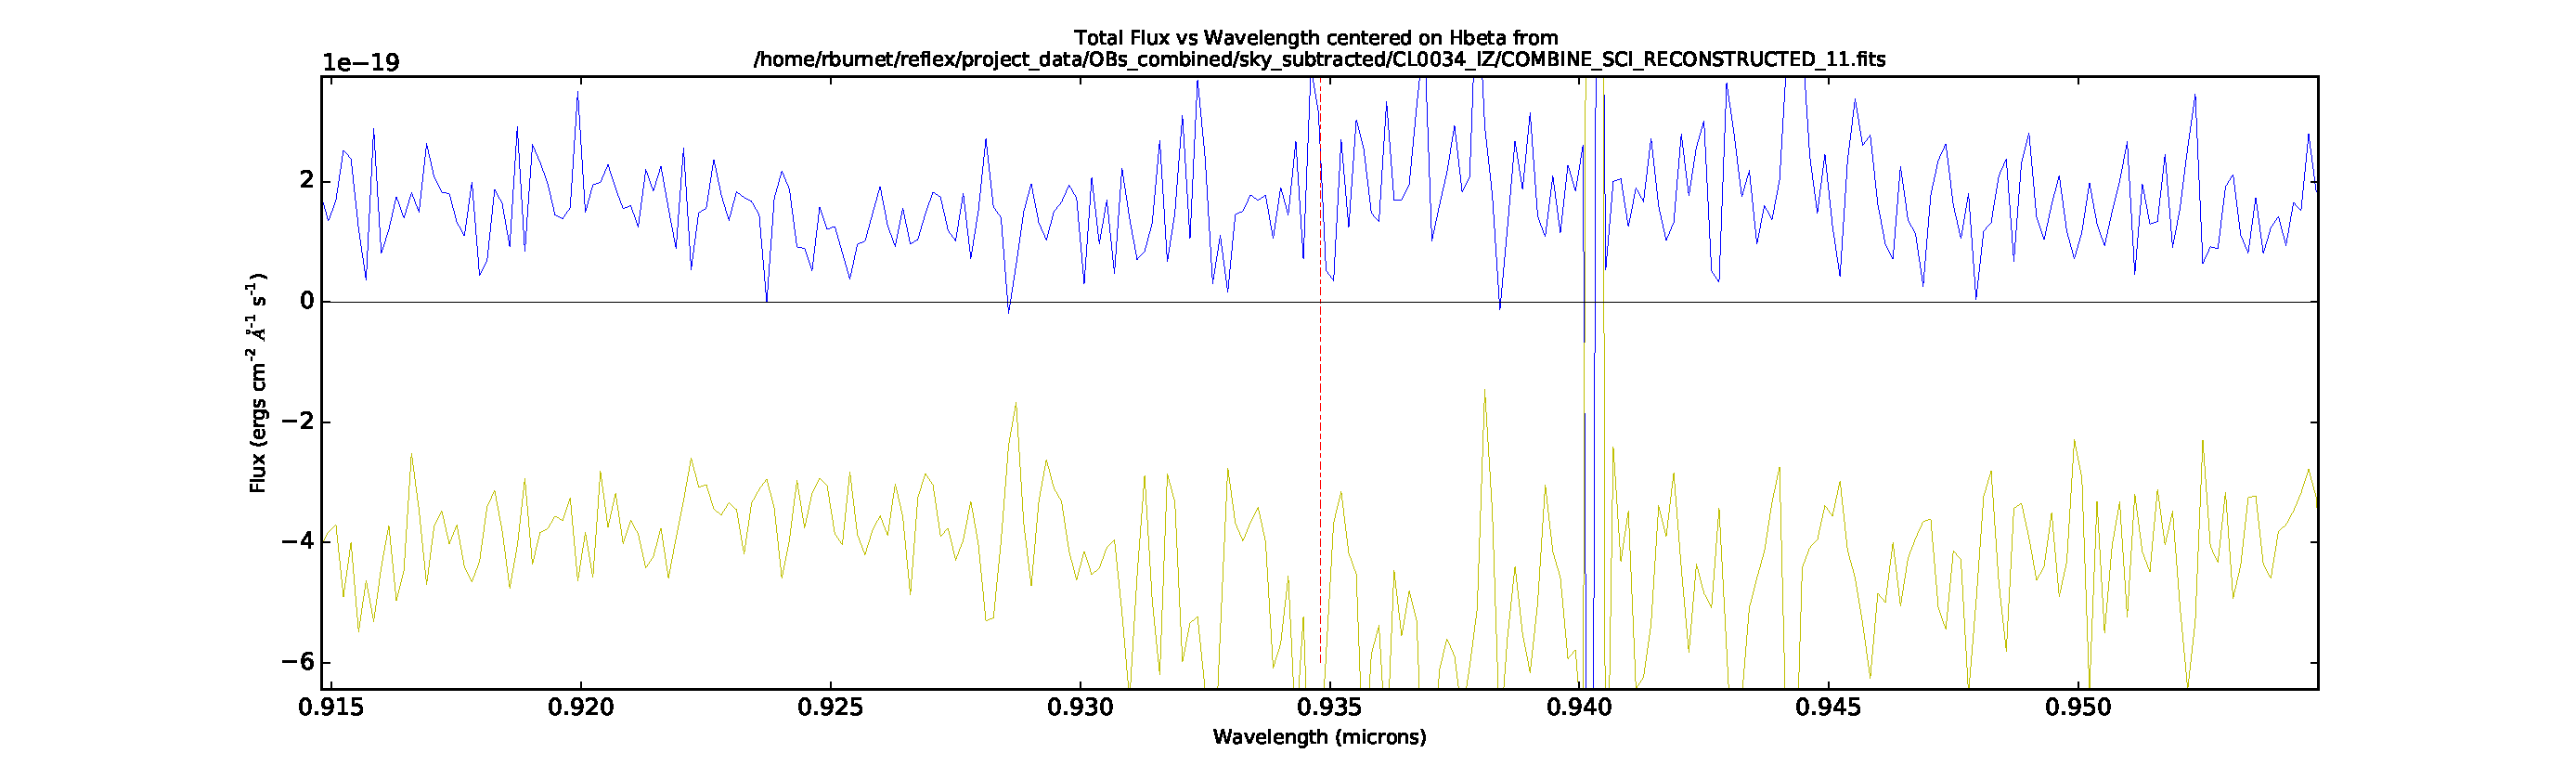
\includegraphics[scale=0.45]{../figures/CL0034_IZ/COMBINE_SCI_RECONSTRUCTED_11_OIII.pdf} \\
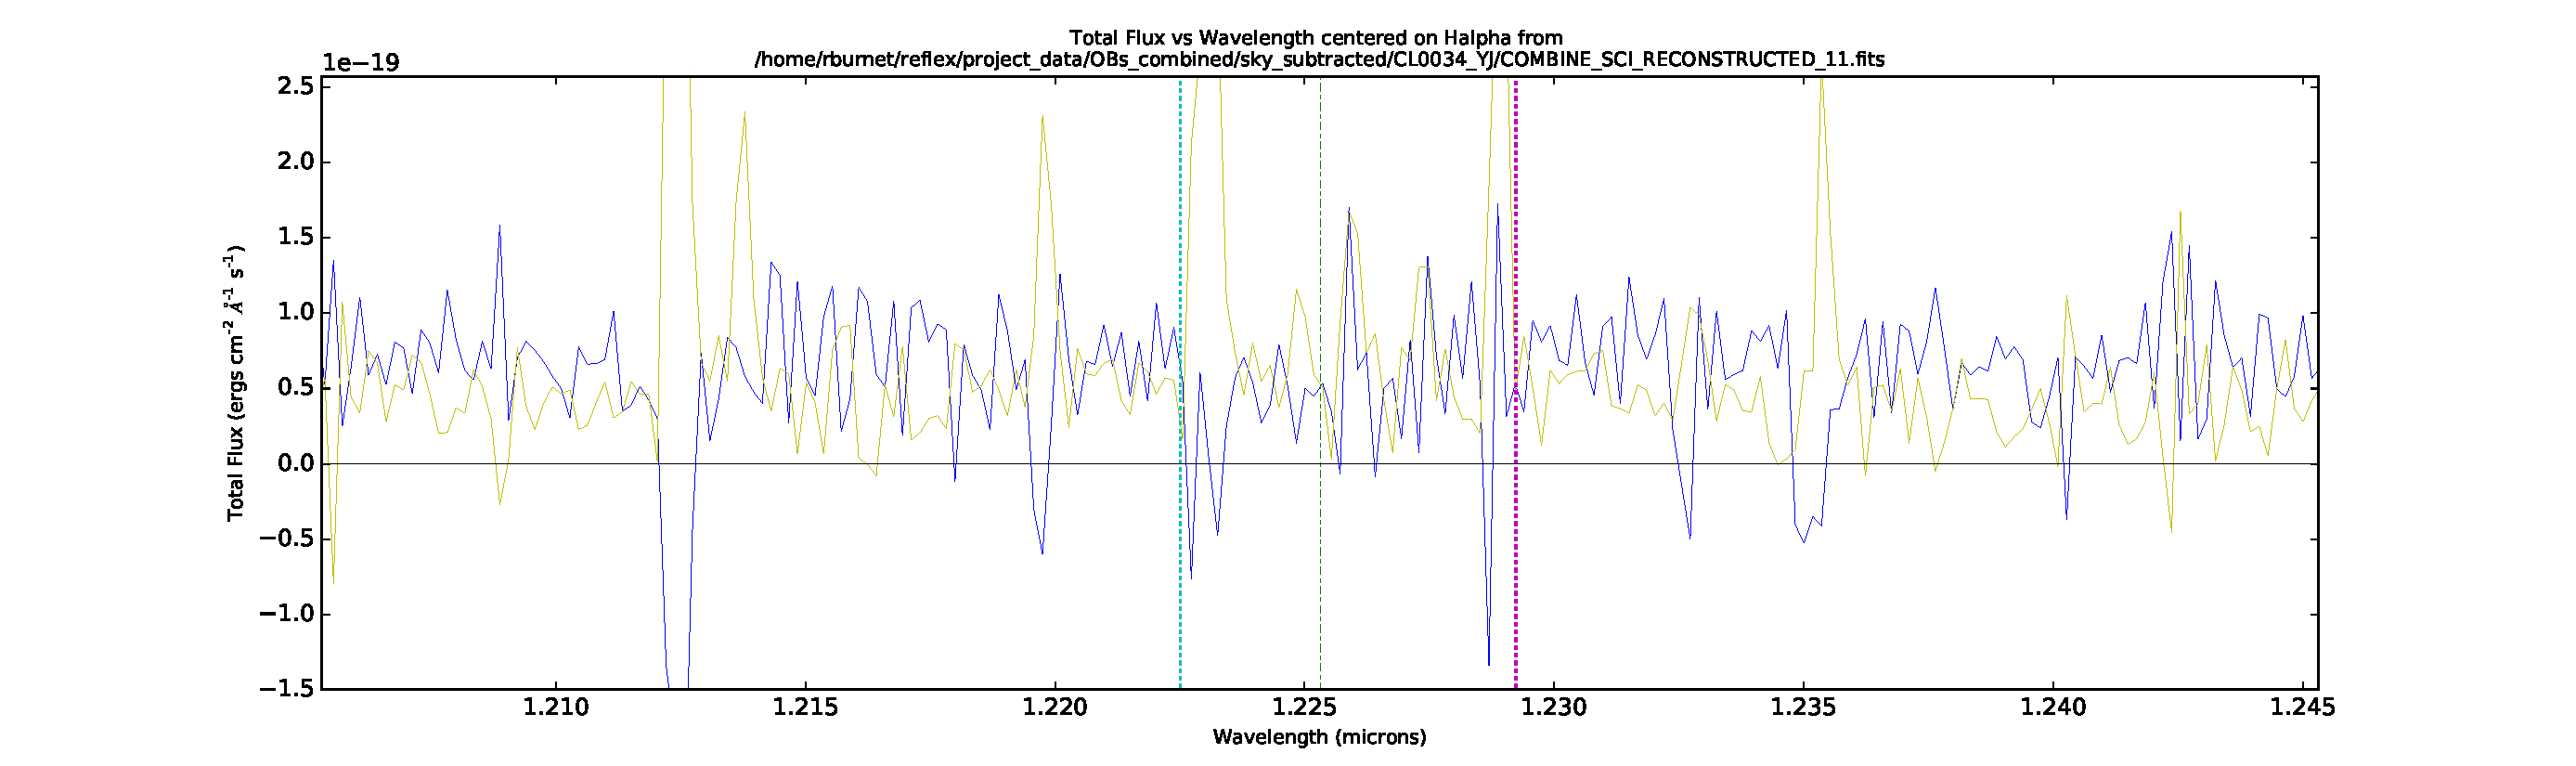
\includegraphics[scale=0.45]{../figures/CL0034_YJ/COMBINE_SCI_RECONSTRUCTED_11_Halpha.pdf}
%\end{tabular} \\
\end{tabular}
\end{center}
\end{table}

\newpage
CL0034 Target 30, Arm 17 \\

\begin{table}[h!]
\begin{center}
\begin{tabular}{ >{\centering\arraybackslash}m{2.5in} >{\centering\arraybackslash}m{2.5in} >{\centering\arraybackslash}m{2.3in}}
HST Image &  Collapsed IZ Image & \\
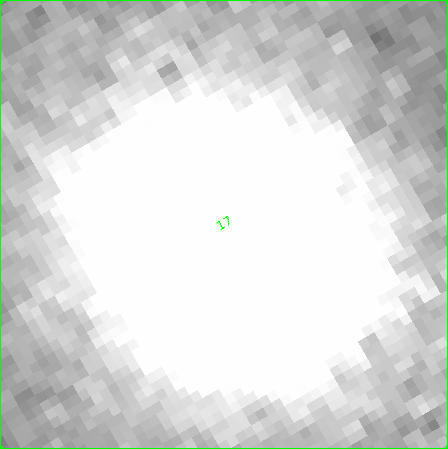
\includegraphics[scale=0.35]{/home/rburnet/S16work/diagnostic_of_objects/figures/HST_images/CL0034/CL0034-Target_30.png} 
&

\includegraphics[scale=0.4]{/home/rburnet/S16work/diagnostic_of_objects/local_sky_subtraction/new_report/figures/CL0034-IZ-Target_30.png} 
&
\begin{tabular}{ l l l }
M$_{\text{IZ, calculated}}$ & = &  20.09\\
M$_{\text{Z, expected}}$ & = & 20.03\\
F(H$\alpha) _{\text{expected}}$ & = & Unknown\\
F(H$\alpha) _{\text{expected, uncorrected}}$ & = & Unknown\\
\end{tabular} \\
\\
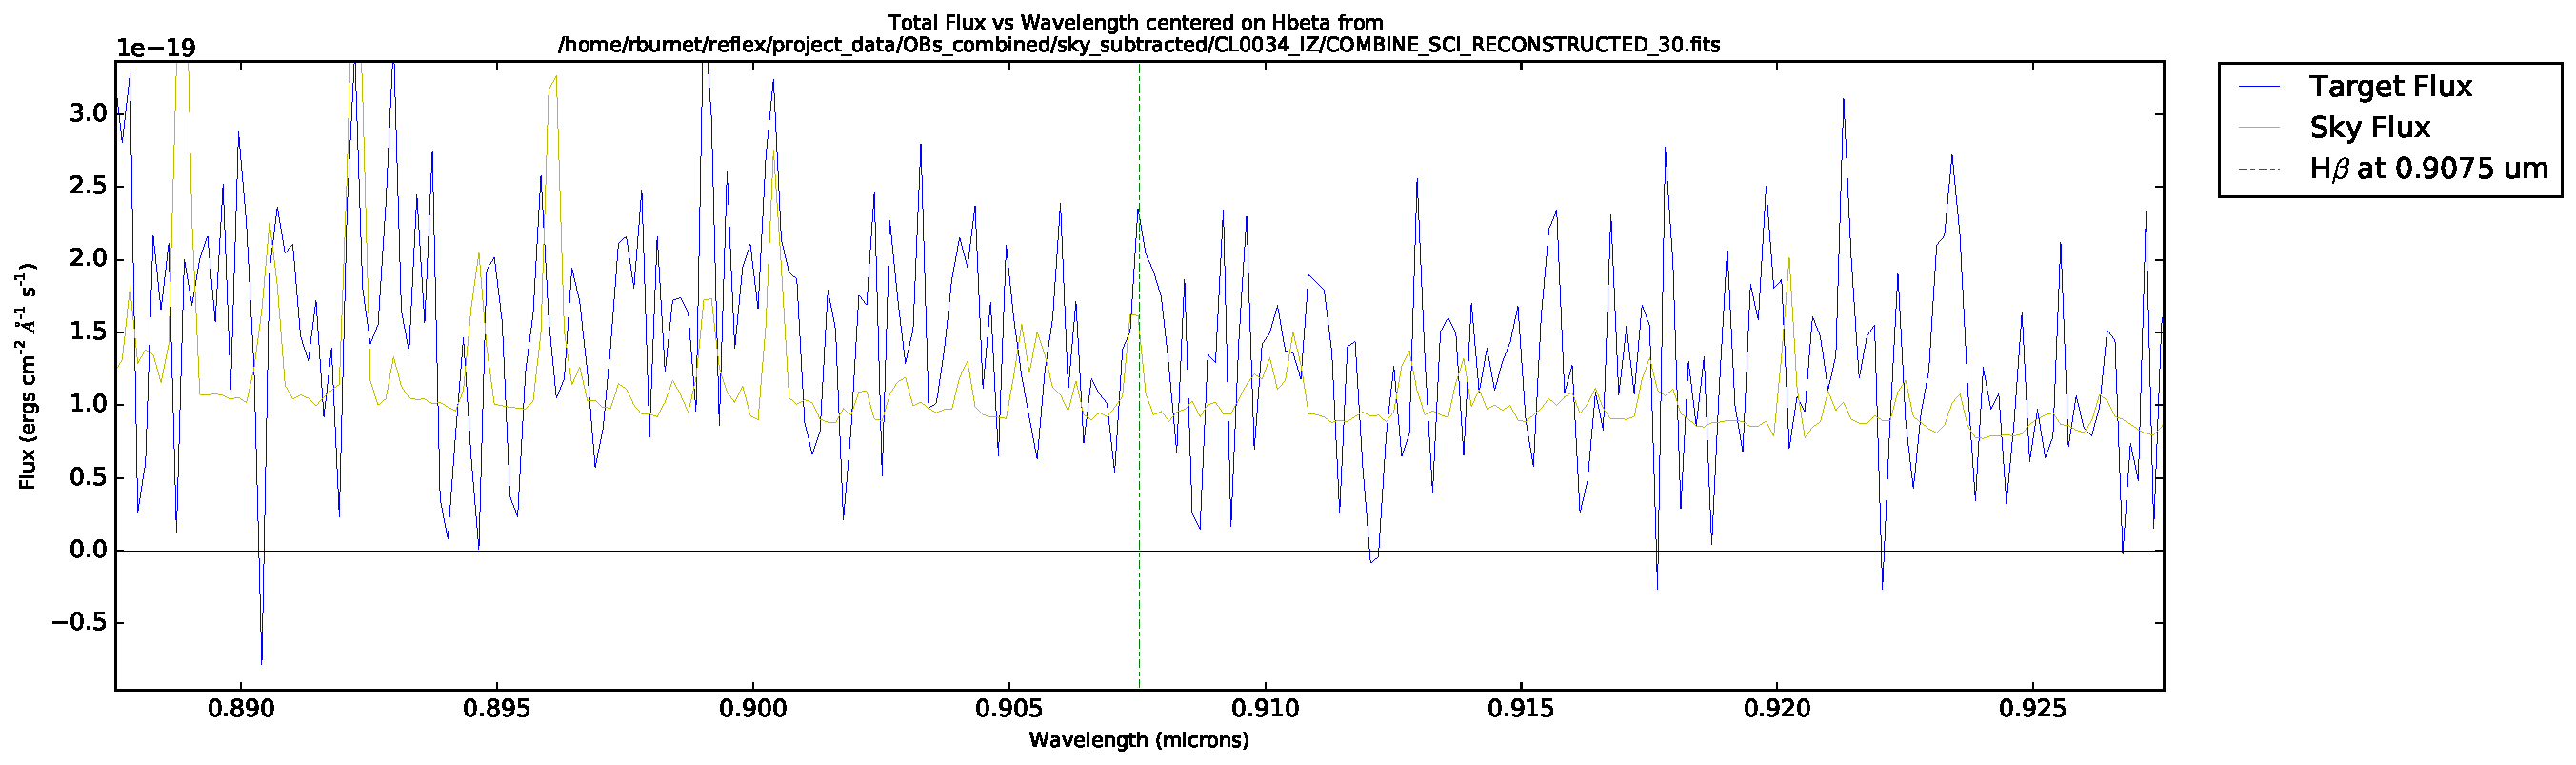
\includegraphics[scale=0.45]{../figures/CL0034_IZ/COMBINE_SCI_RECONSTRUCTED_30_Hbeta.pdf} \\
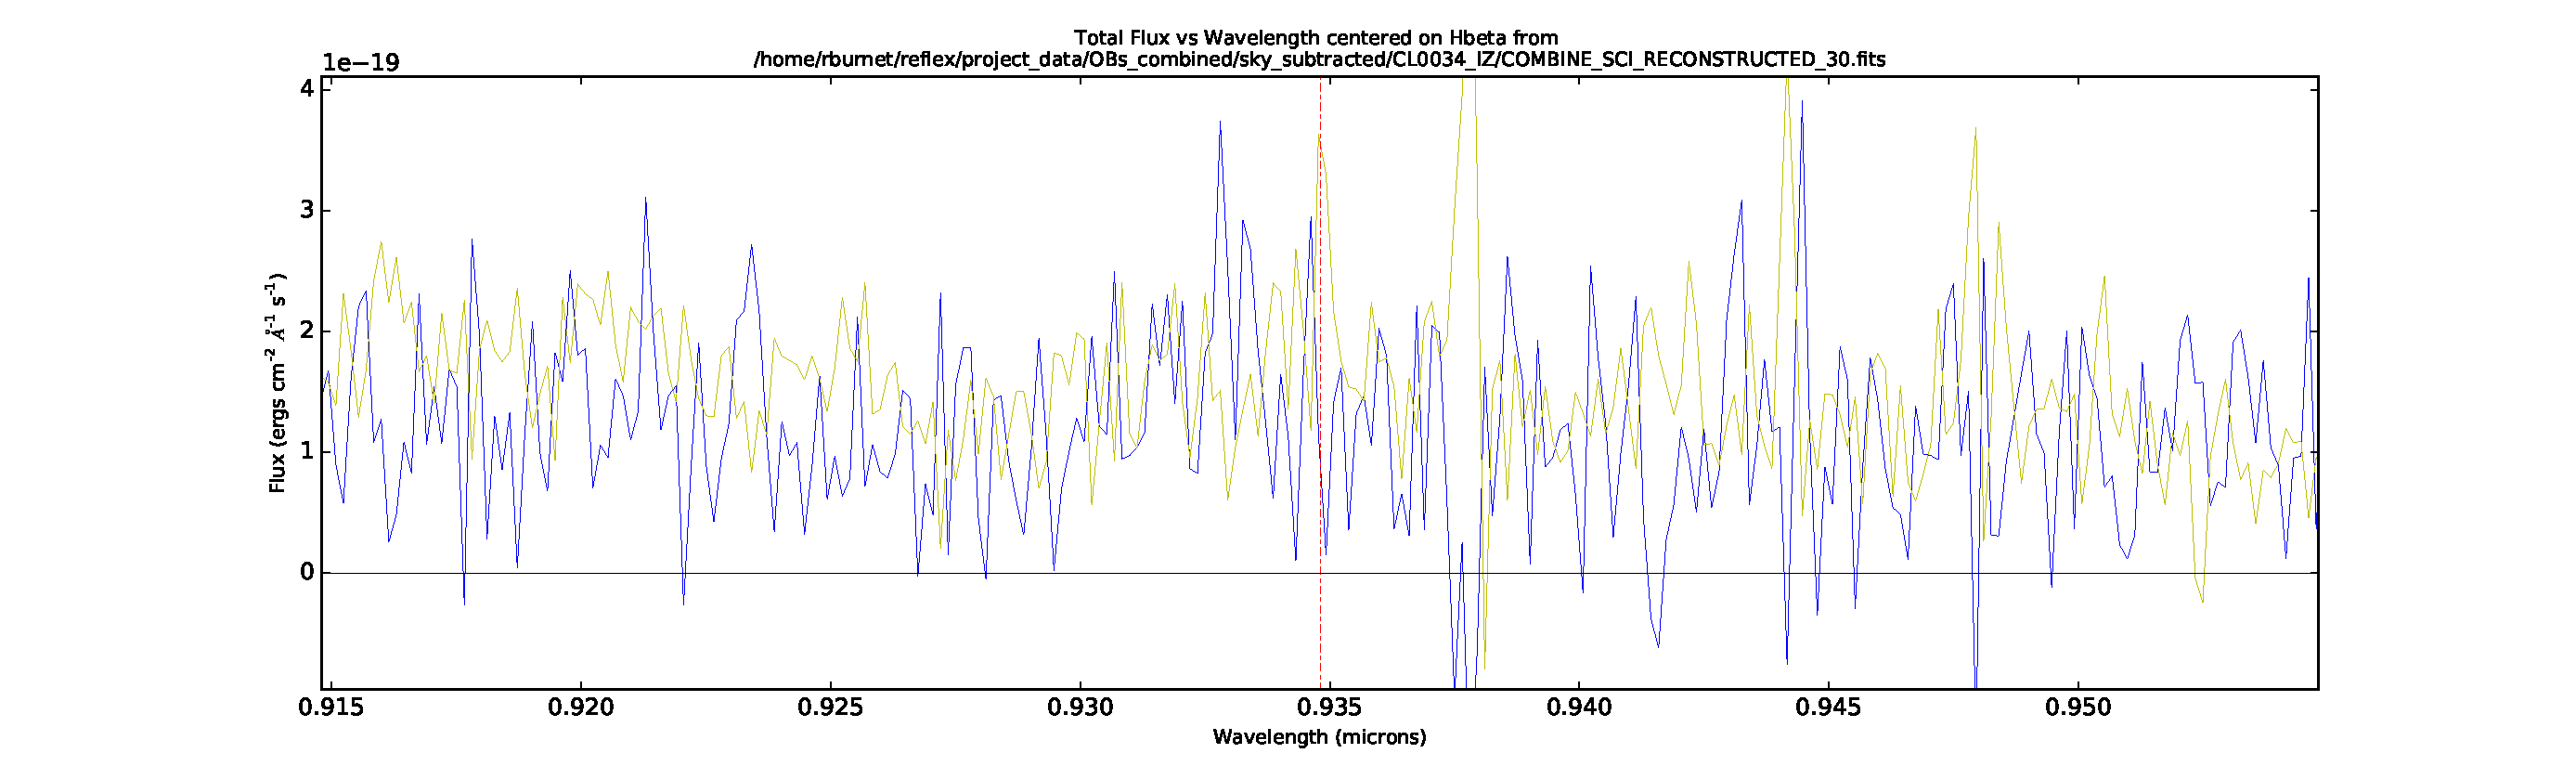
\includegraphics[scale=0.45]{../figures/CL0034_IZ/COMBINE_SCI_RECONSTRUCTED_30_OIII.pdf} 
\end{tabular}
\end{center}
\end{table}

\newpage

CL0034 Target 5, Arm 10 \\

\begin{table}[h!]
\begin{center}
\begin{tabular}{ >{\centering\arraybackslash}m{2.5in} >{\centering\arraybackslash}m{2.5in} >{\centering\arraybackslash}m{2.5in} >{\centering\arraybackslash}m{2.3in}}
HST Image & Collapsed YJ Image &  Collapsed IZ Image & \\
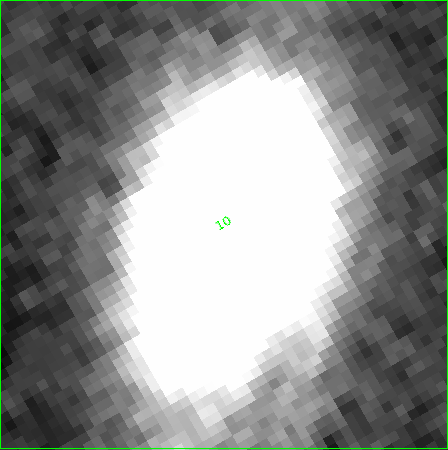
\includegraphics[scale=0.35]{/home/rburnet/S16work/diagnostic_of_objects/figures/HST_images/CL0034/CL0034-Target_5.png} 
& 
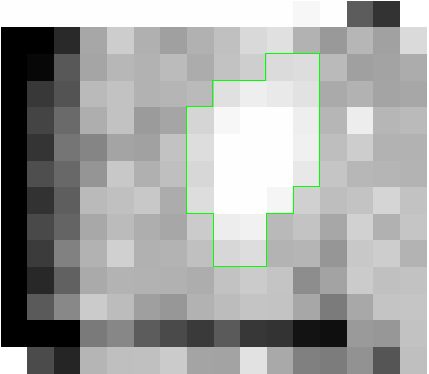
\includegraphics[scale=0.4]{/home/rburnet/S16work/diagnostic_of_objects/local_sky_subtraction/new_report/figures/CL0034-IZ-Target_5.png} 
&
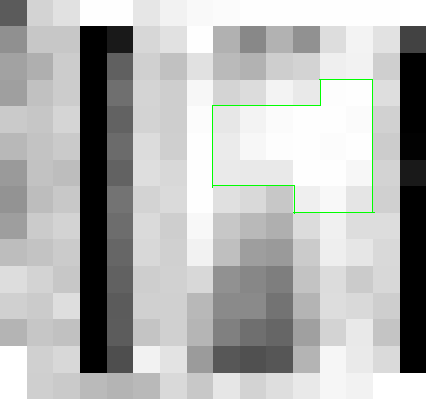
\includegraphics[scale=0.4]{/home/rburnet/S16work/diagnostic_of_objects/local_sky_subtraction/new_report/figures/CL0034-YJ-Target_5.png} 
\\
&
\begin{tabular}{ l l l }
M$_{\text{IZ, calculated}}$ & = &  21.24\\
M$_{\text{YJ, calculated}}$ & = &  20.87\\
M$_{\text{Z, expected}}$ & = & 20.46\\
F(H$\alpha) _{\text{expected}}$ & = & 2.561e-15\\
F(H$\alpha) _{\text{expected, uncorrected}}$ & = & 8.440e-16\\
\end{tabular} \\
\\
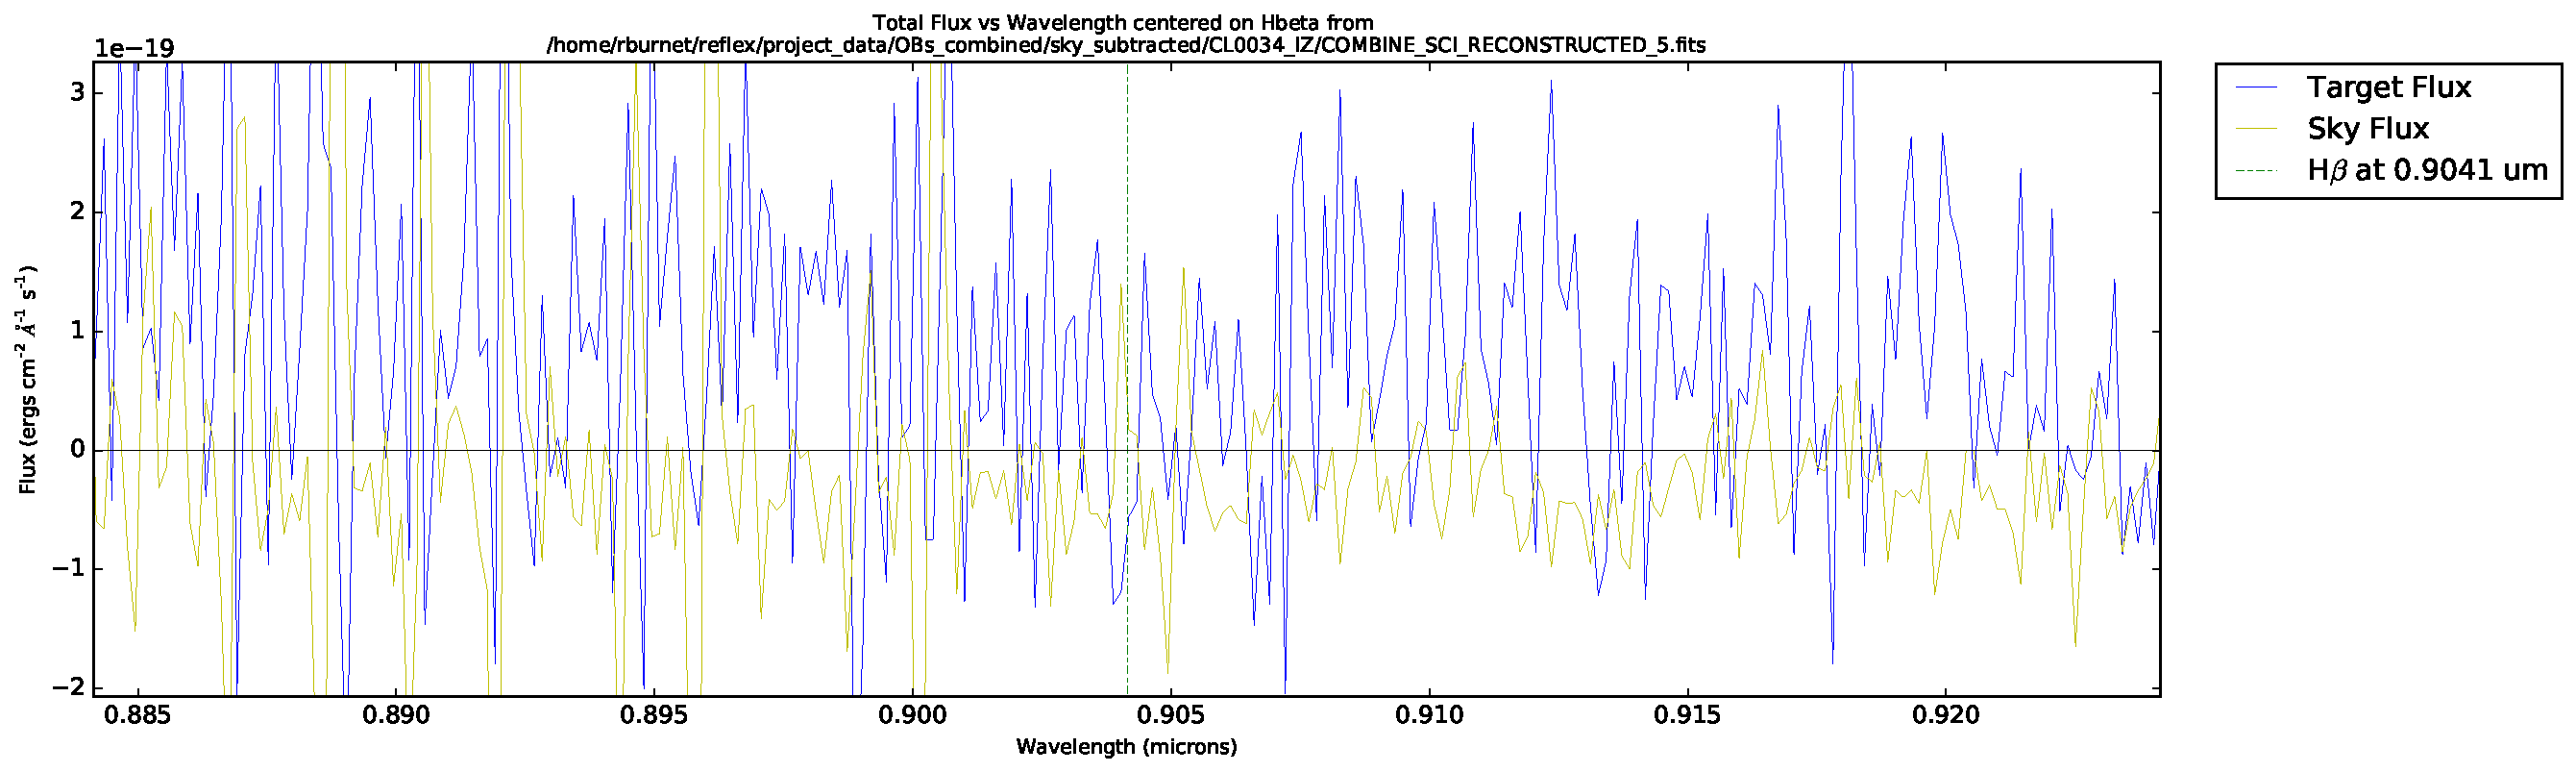
\includegraphics[scale=0.45]{../figures/CL0034_IZ/COMBINE_SCI_RECONSTRUCTED_5_Hbeta.pdf} \\
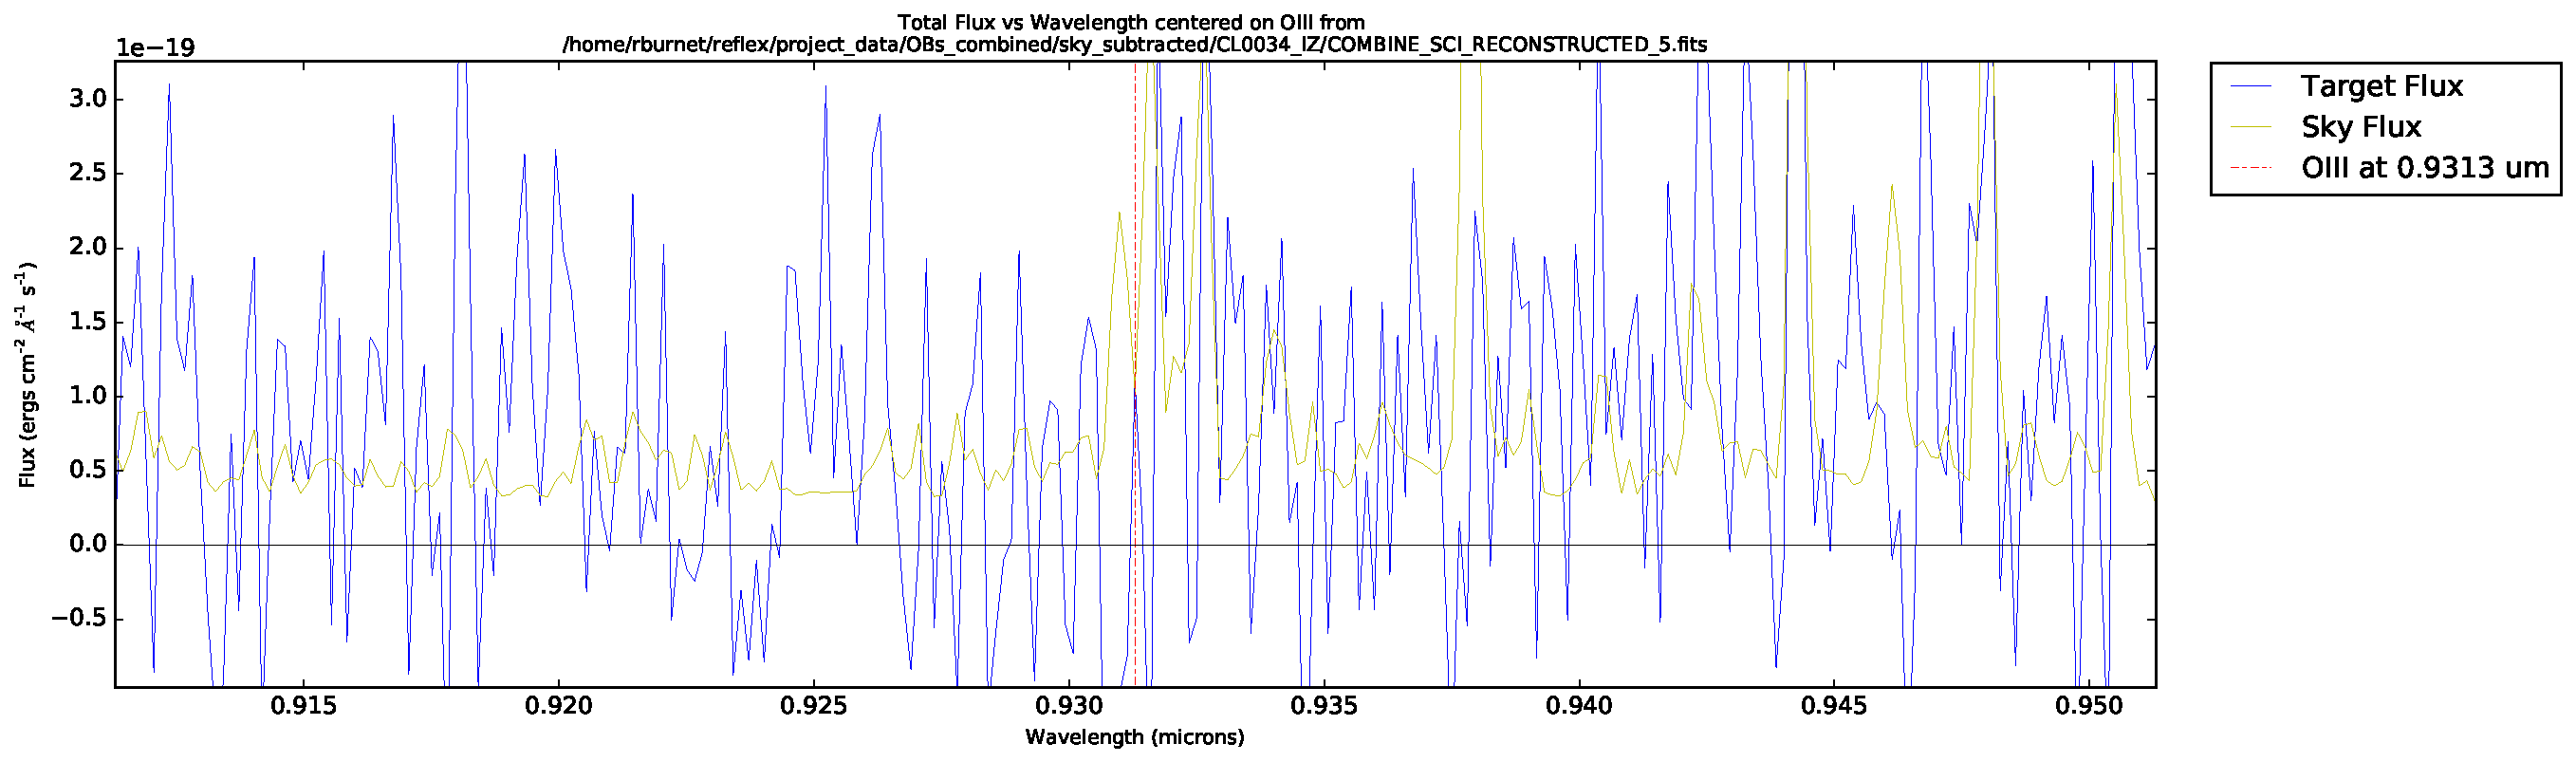
\includegraphics[scale=0.45]{../figures/CL0034_IZ/COMBINE_SCI_RECONSTRUCTED_5_OIII.pdf} \\
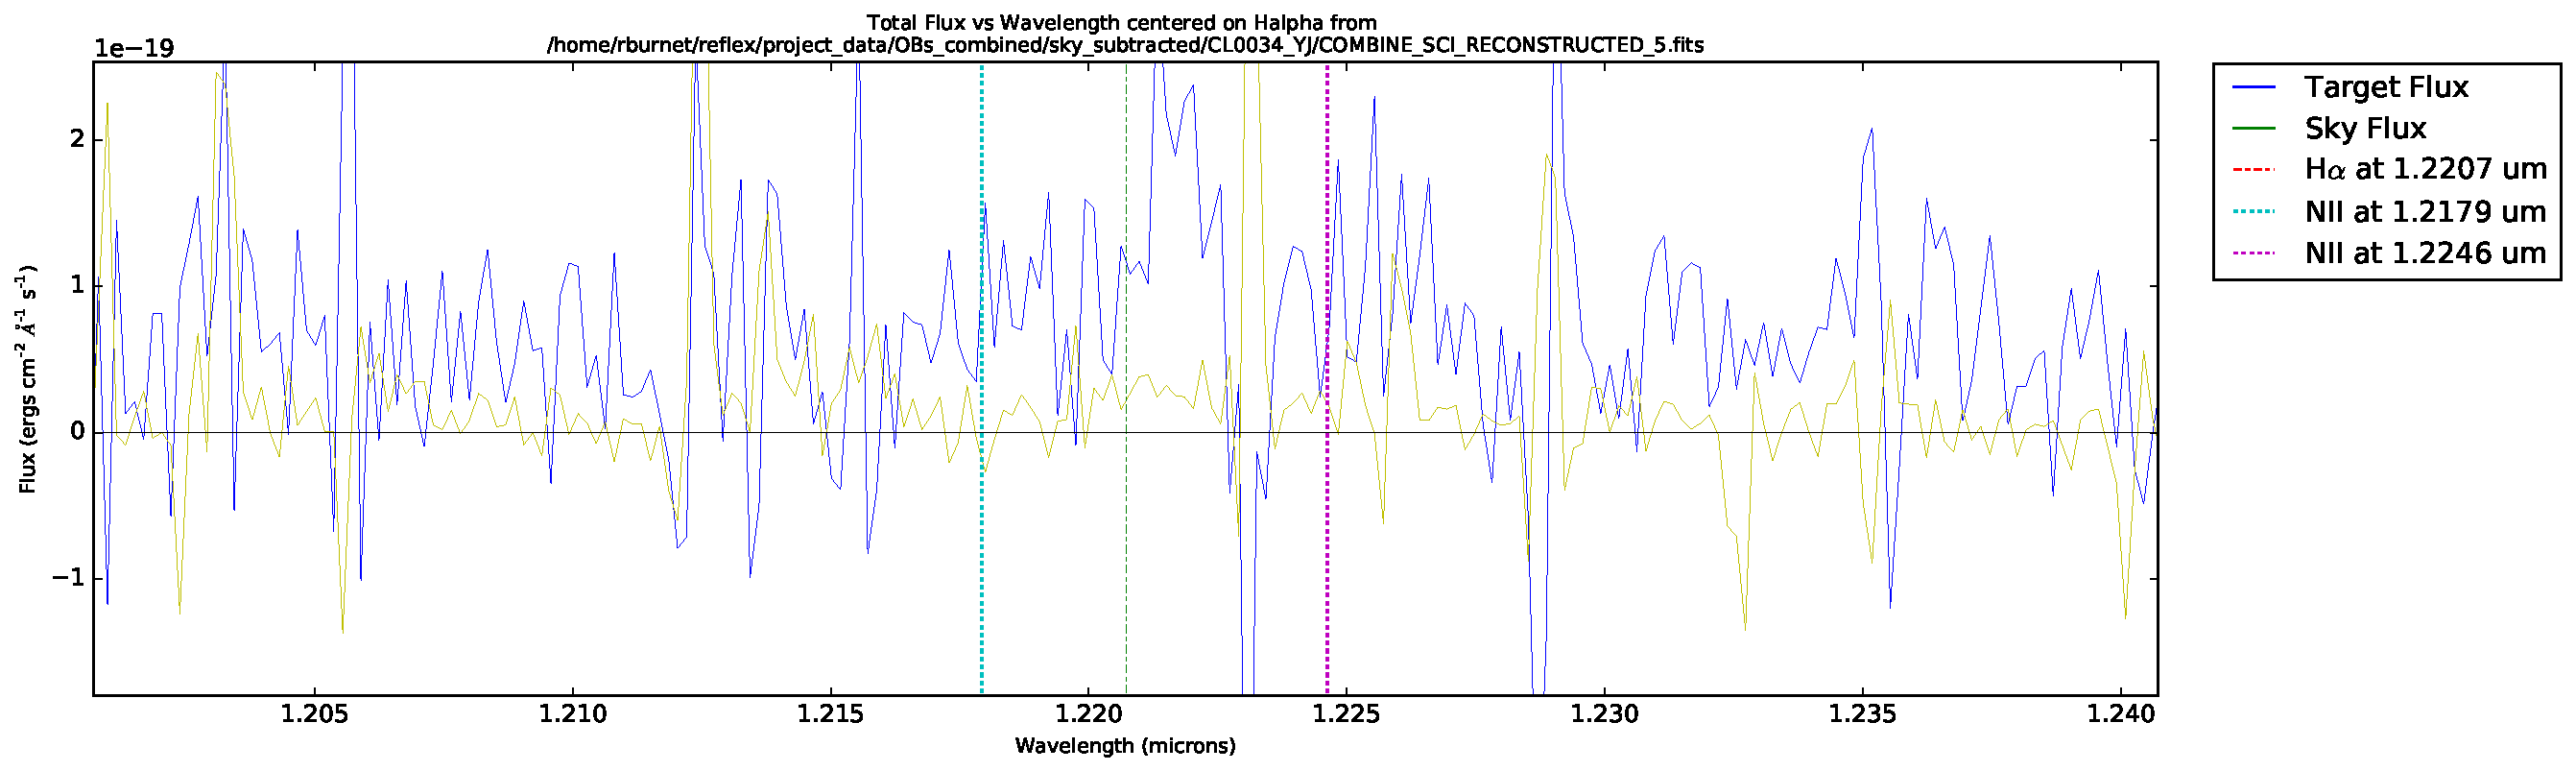
\includegraphics[scale=0.45]{../figures/CL0034_YJ/COMBINE_SCI_RECONSTRUCTED_5_Halpha.pdf}
\end{tabular}
\end{center}
\end{table}

\newpage
CL0034 Target 12, Arm 15 \\

\begin{table}[h!]
\begin{center}
\begin{tabular}{ >{\centering\arraybackslash}m{2.5in} >{\centering\arraybackslash}m{2.5in} >{\centering\arraybackslash}m{2.5in} >{\centering\arraybackslash}m{2.3in}}
HST Image & Collapsed YJ Image &  Collapsed IZ Image & \\
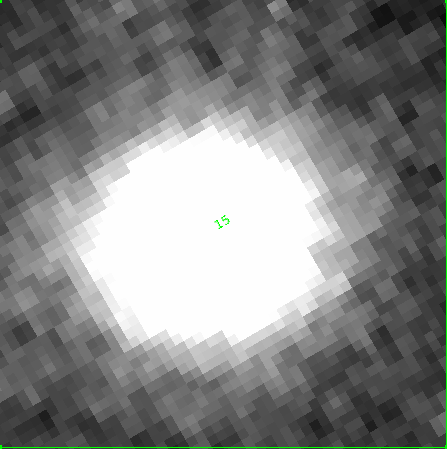
\includegraphics[scale=0.35]{/home/rburnet/S16work/diagnostic_of_objects/figures/HST_images/CL0034/CL0034-Target_12.png} 
&
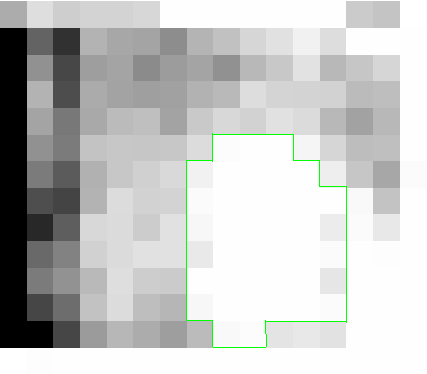
\includegraphics[scale=0.4]{/home/rburnet/S16work/diagnostic_of_objects/local_sky_subtraction/new_report/figures/CL0034-IZ-Target_12.png}
&

\includegraphics[scale=0.4]{/home/rburnet/S16work/diagnostic_of_objects/local_sky_subtraction/new_report/figures/CL0034-YJ-Target_12.png} 
\\
&
\begin{tabular}{ l l l }
M$_{\text{IZ, calculated}}$ & = &  20.71\\
M$_{\text{YJ, calculated}}$ & = &  20.09\\
M$_{\text{Z, expected}}$ & = & 20.55\\
F(H$\alpha) _{\text{expected}}$ & = & 1.379e-15\\
F(H$\alpha) _{\text{expected, uncorrected}}$ & = & 4.636e-16\\
\end{tabular} \\
\\
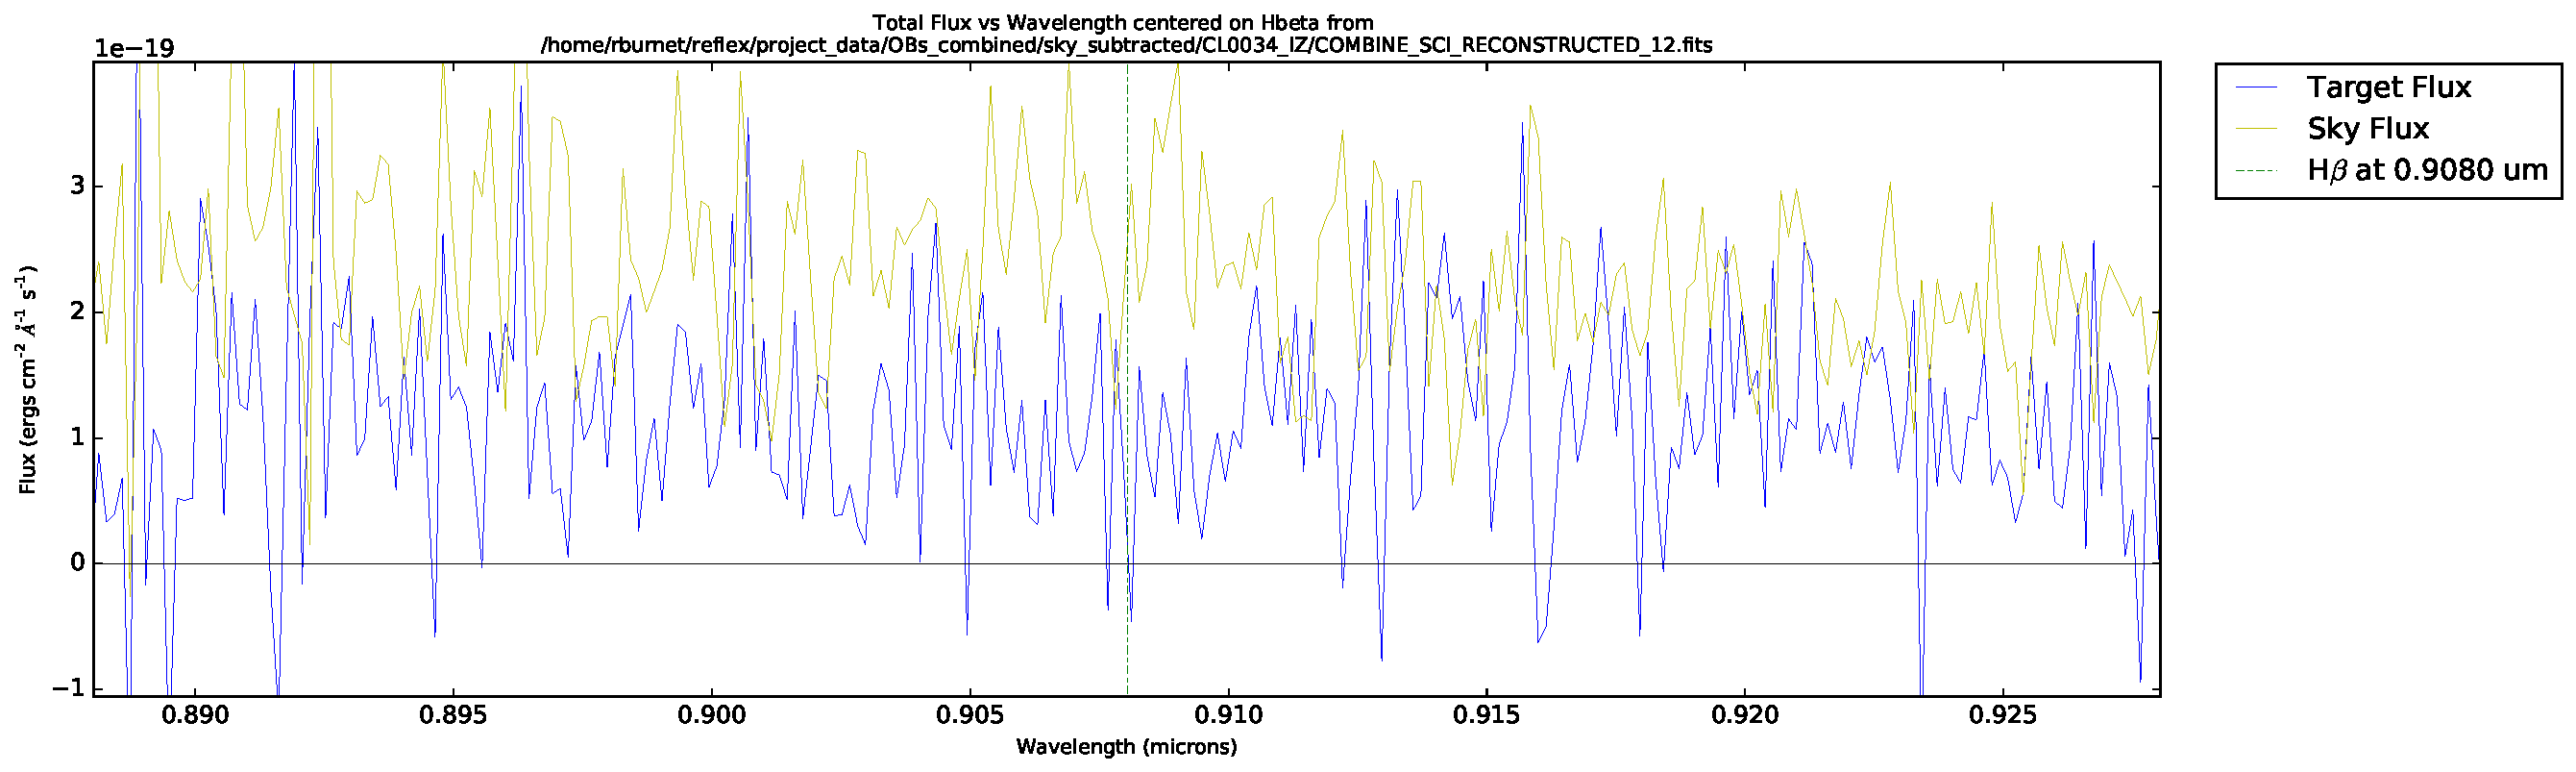
\includegraphics[scale=0.45]{../figures/CL0034_IZ/COMBINE_SCI_RECONSTRUCTED_12_Hbeta.pdf} \\
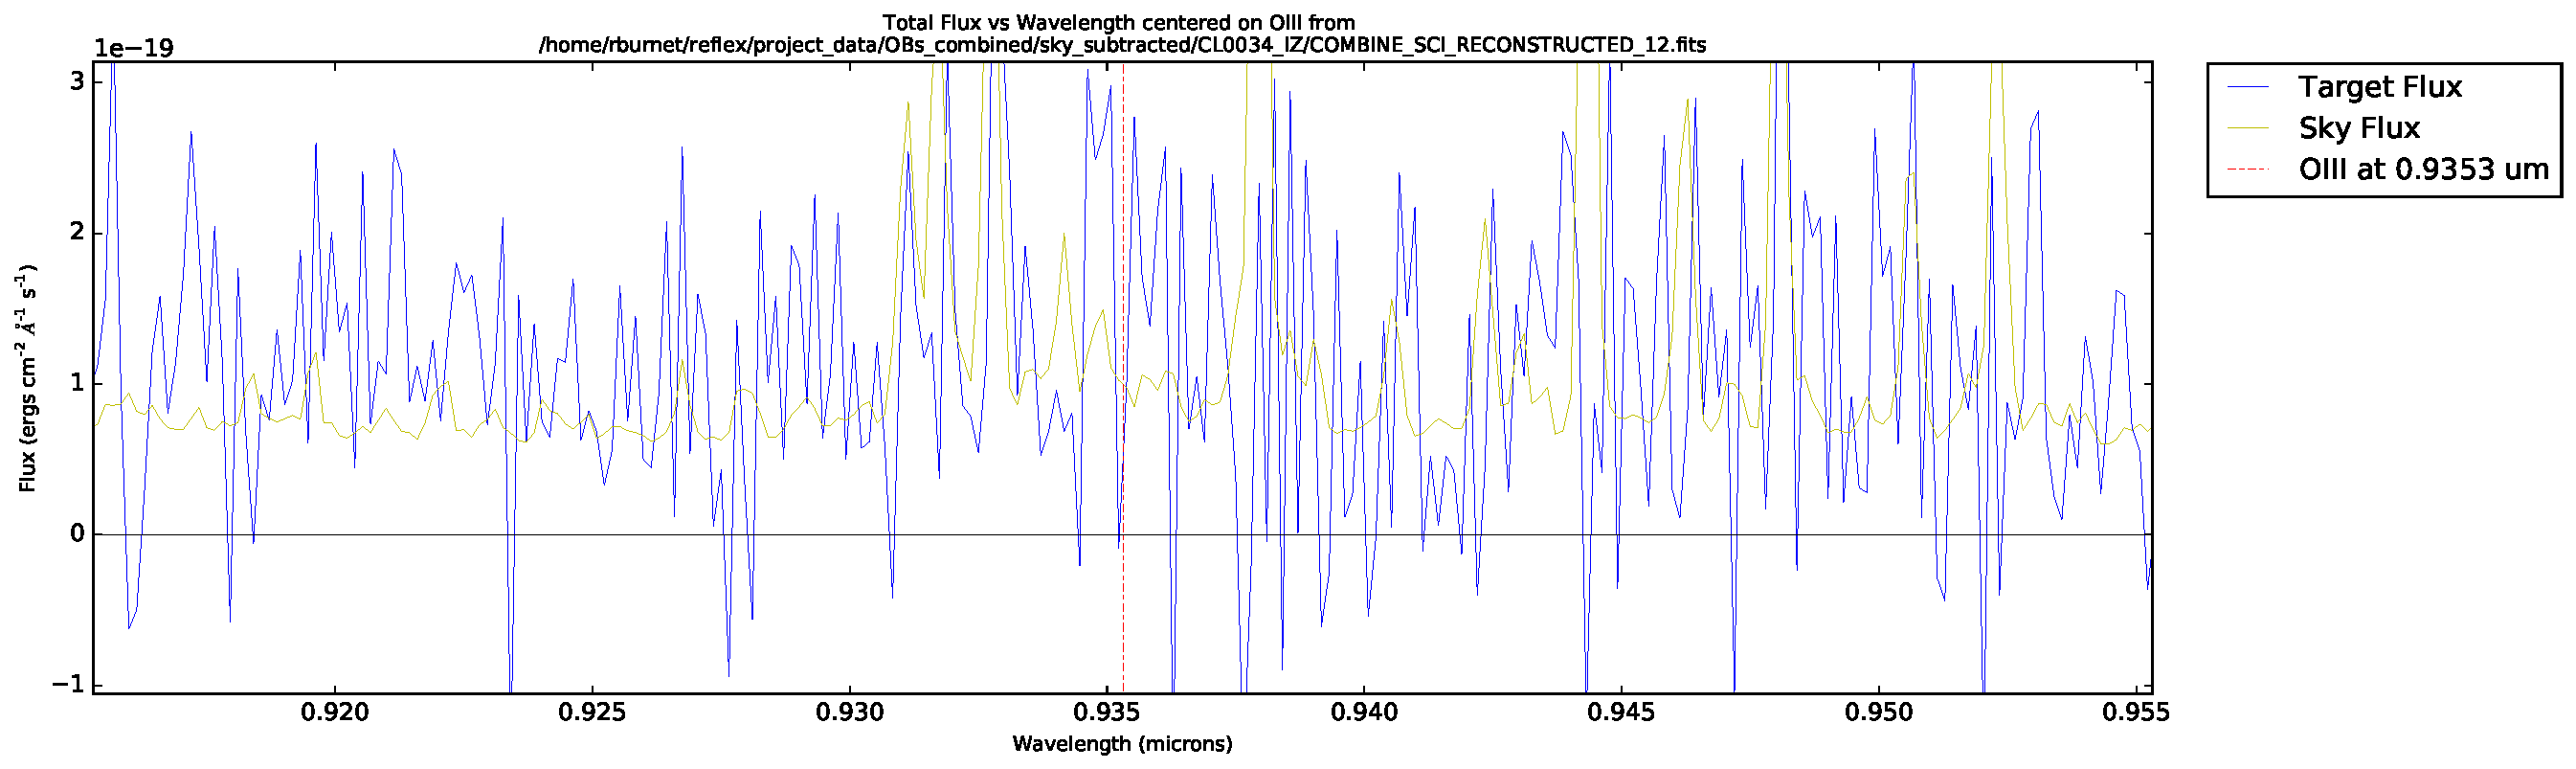
\includegraphics[scale=0.45]{../figures/CL0034_IZ/COMBINE_SCI_RECONSTRUCTED_12_OIII.pdf} \\
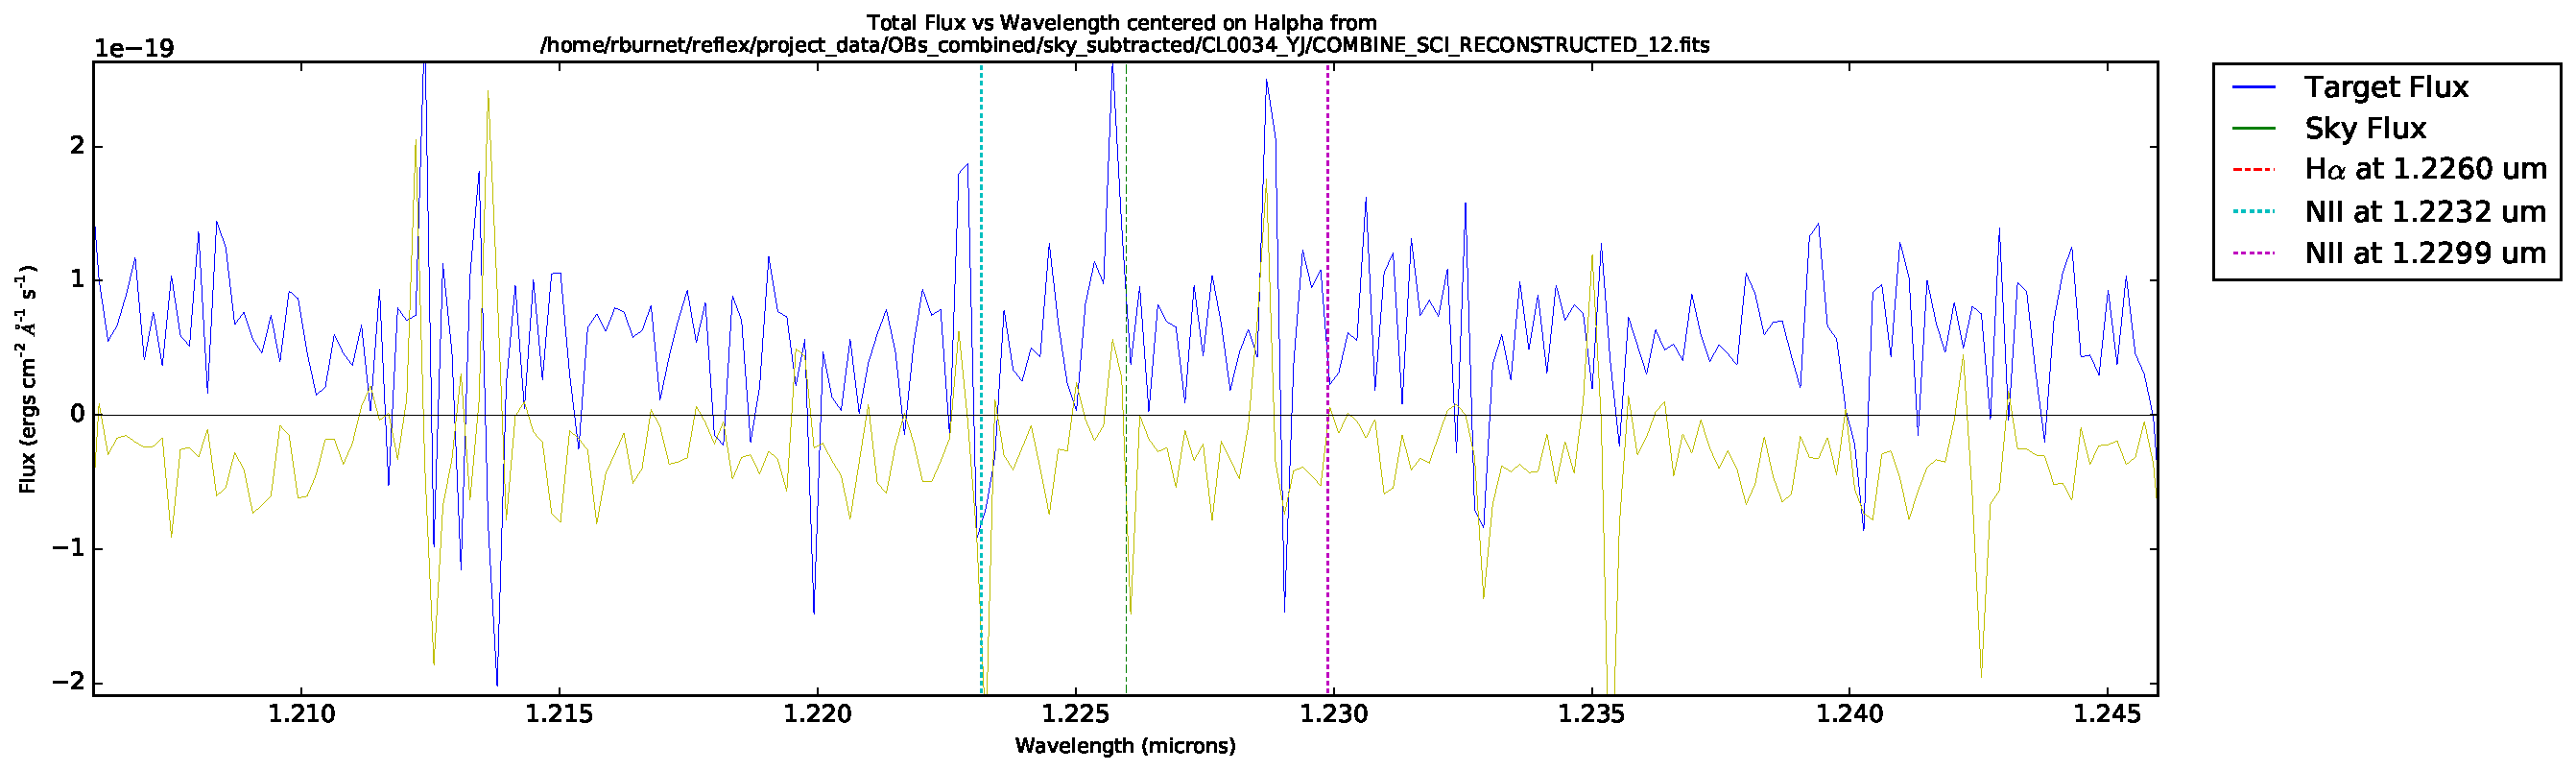
\includegraphics[scale=0.45]{../figures/CL0034_YJ/COMBINE_SCI_RECONSTRUCTED_12_Halpha.pdf}
\end{tabular}
\end{center}
\end{table}

\newpage 

CL0034 Target 31, Arm 18 \\

\begin{table}[h!]
\begin{center}
\begin{tabular}{ >{\centering\arraybackslash}m{2.5in} >{\centering\arraybackslash}m{2.5in} >{\centering\arraybackslash}m{2.5in} >{\centering\arraybackslash}m{2.3in}}
HST Image & Collapsed YJ Image &  Collapsed IZ Image & \\
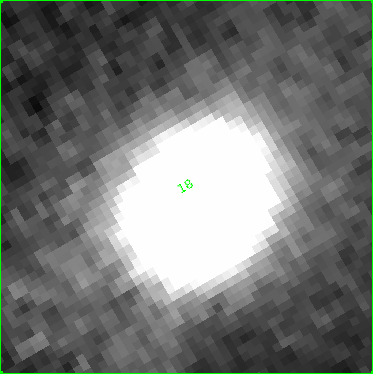
\includegraphics[scale=0.45]{/home/rburnet/S16work/diagnostic_of_objects/figures/HST_images/CL0034/CL0034-Target_31.png} 
&

\includegraphics[scale=0.4]{/home/rburnet/S16work/diagnostic_of_objects/local_sky_subtraction/new_report/figures/CL0034-IZ-Target_31.png}  
&
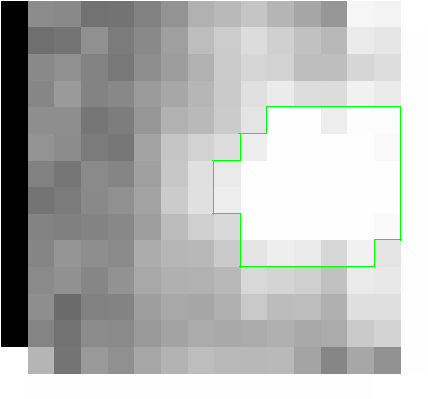
\includegraphics[scale=0.4]{/home/rburnet/S16work/diagnostic_of_objects/local_sky_subtraction/new_report/figures/CL0034-YJ-Target_31.png} 
\\
&
\begin{tabular}{ l l l }
M$_{\text{IZ, calculated}}$ & = &  20.33\\
M$_{\text{YJ, calculated}}$ & = &  20.40\\
M$_{\text{Z, expected}}$ & = & 20.84\\
F(H$\alpha) _{\text{expected}}$ & = & Unknown\\
F(H$\alpha) _{\text{expected, uncorrected}}$ & = & Unknown\\
\end{tabular} \\
\\
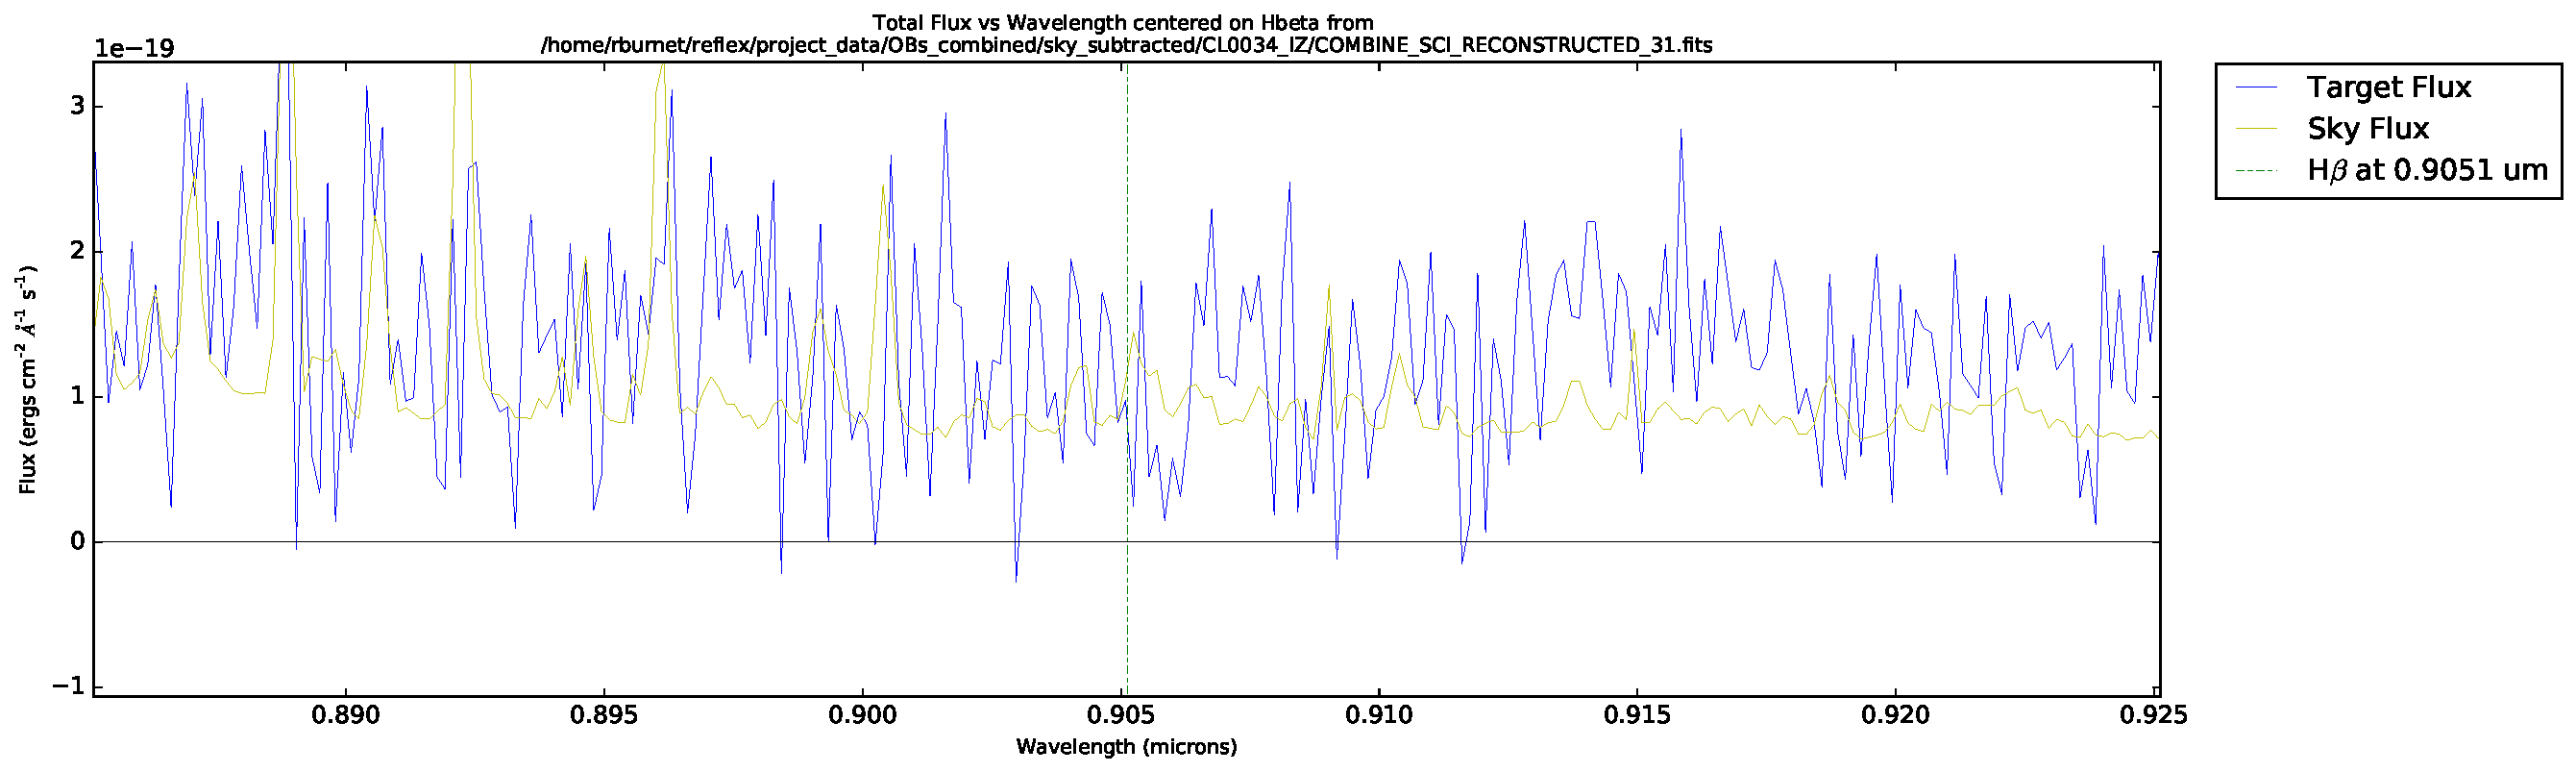
\includegraphics[scale=0.45]{../figures/CL0034_IZ/COMBINE_SCI_RECONSTRUCTED_31_Hbeta.pdf} \\
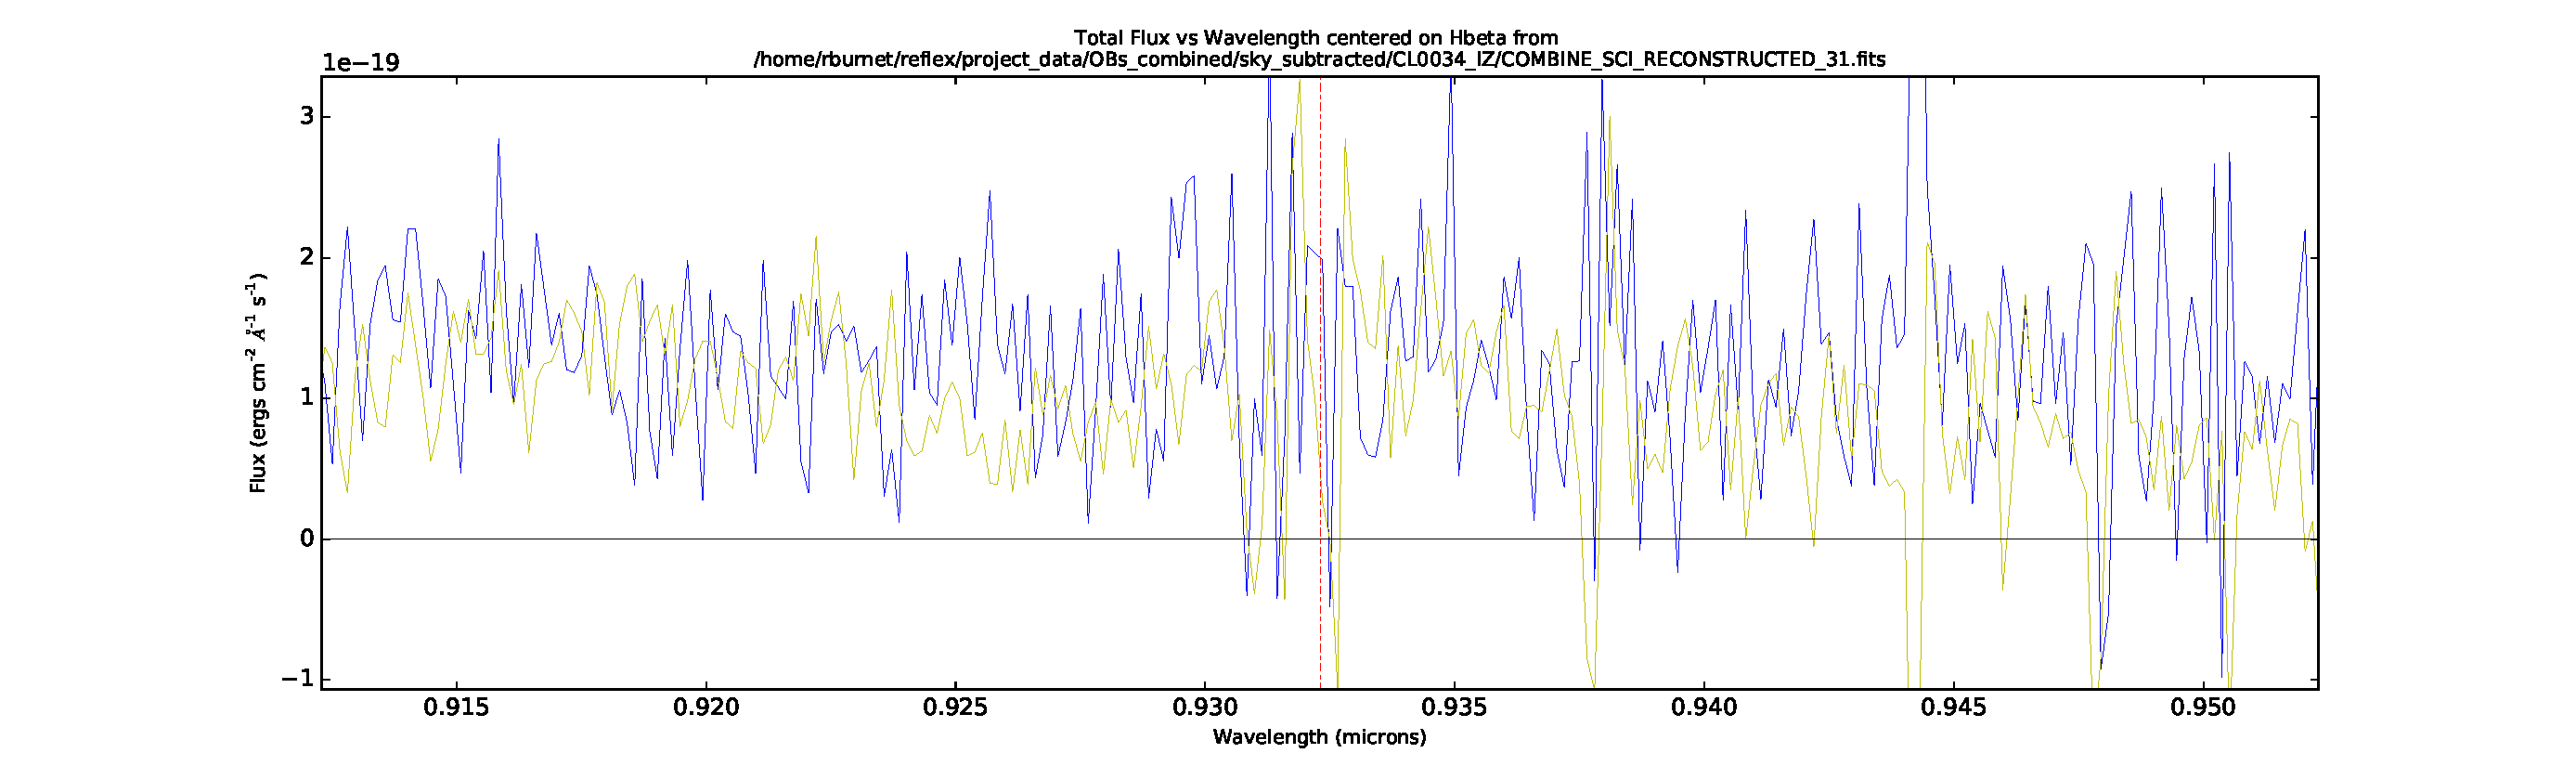
\includegraphics[scale=0.45]{../figures/CL0034_IZ/COMBINE_SCI_RECONSTRUCTED_31_OIII.pdf} \\
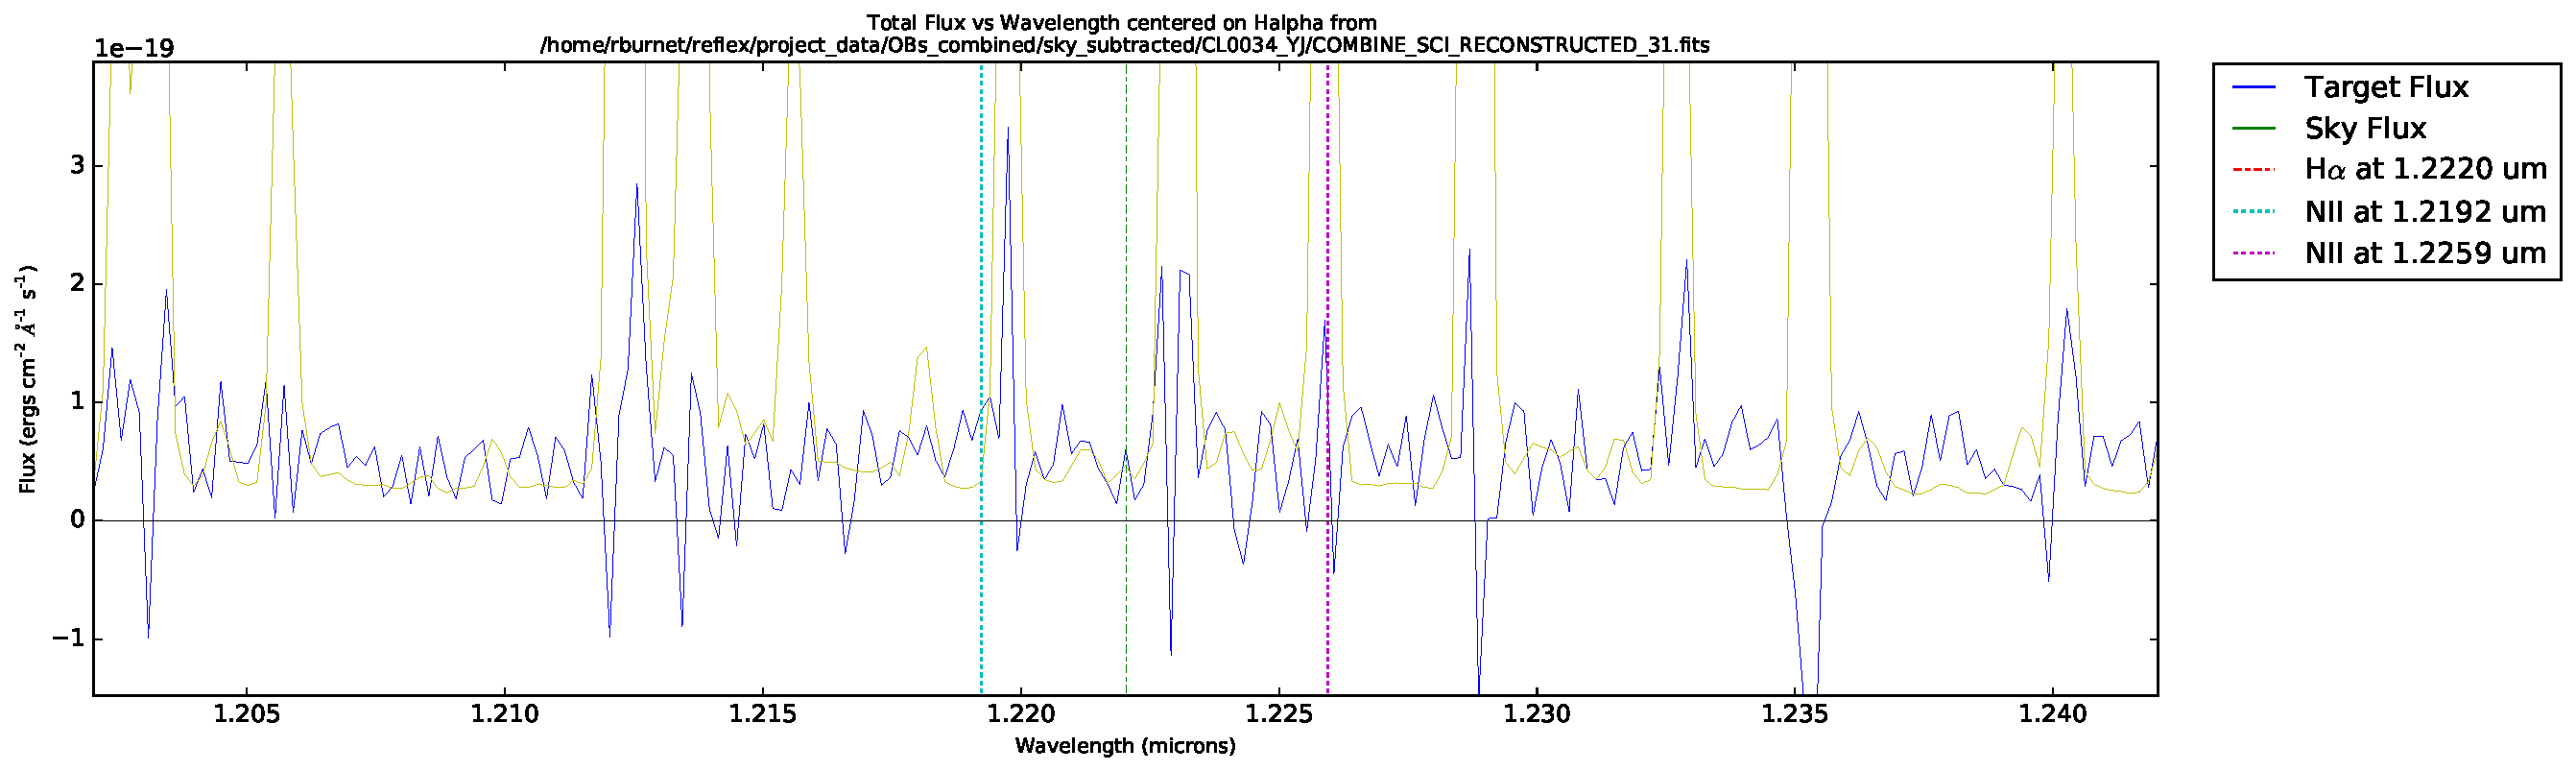
\includegraphics[scale=0.45]{../figures/CL0034_YJ/COMBINE_SCI_RECONSTRUCTED_31_Halpha.pdf}
\end{tabular}
\end{center}
\end{table}

\newpage
CL0034 Target 7, Arm 16 \\

\begin{table}[h!]
\begin{center}
\begin{tabular}{ >{\centering\arraybackslash}m{2.5in} >{\centering\arraybackslash}m{2.5in} >{\centering\arraybackslash}m{2.5in} >{\centering\arraybackslash}m{2.3in}}
HST Image & Collapsed YJ Image &  Collapsed IZ Image & \\
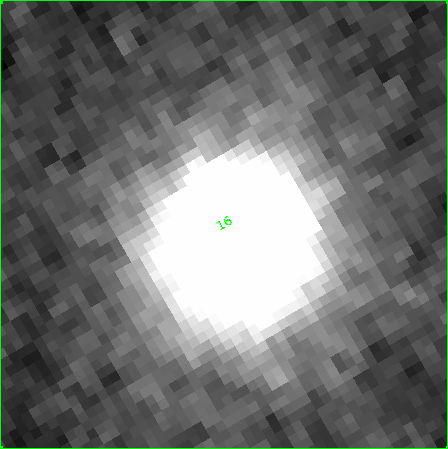
\includegraphics[scale=0.35]{/home/rburnet/S16work/diagnostic_of_objects/figures/HST_images/CL0034/CL0034-Target_7.png} 
&
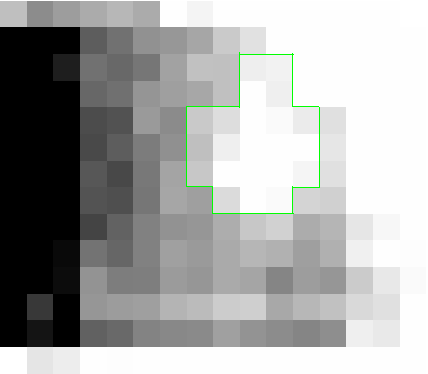
\includegraphics[scale=0.4]{/home/rburnet/S16work/diagnostic_of_objects/local_sky_subtraction/new_report/figures/CL0034-IZ-Target_7.png} 
&

\includegraphics[scale=0.4]{/home/rburnet/S16work/diagnostic_of_objects/local_sky_subtraction/new_report/figures/CL0034-YJ-Target_7.png} 
\\
&
\begin{tabular}{ l l l }
M$_{\text{IZ, calculated}}$ & = &  21.67\\
M$_{\text{YJ, calculated}}$ & = &  20.53\\
M$_{\text{Z, expected}}$ & = & 21.06\\
F(H$\alpha) _{\text{expected}}$ & = & 3.570e-16\\
F(H$\alpha) _{\text{expected, uncorrected}}$ & = & 1.249e-16\\
\end{tabular} \\
\\
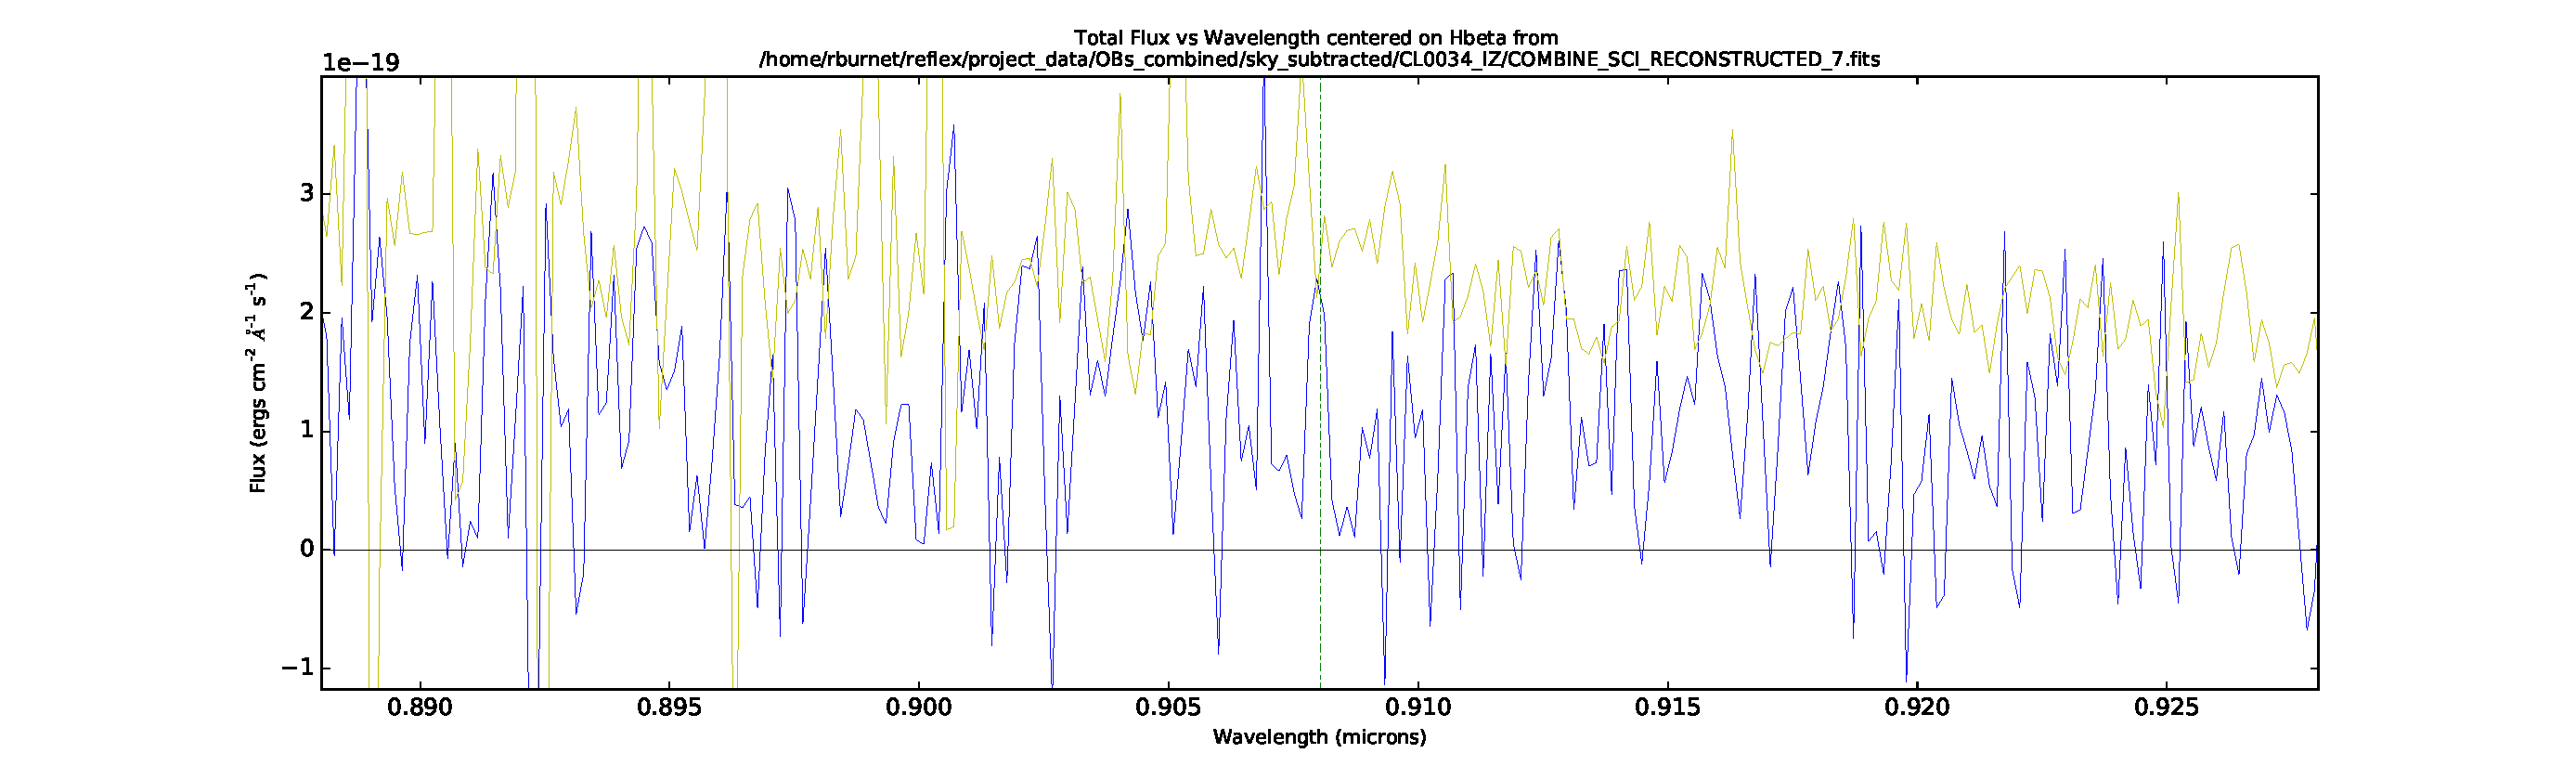
\includegraphics[scale=0.45]{../figures/CL0034_IZ/COMBINE_SCI_RECONSTRUCTED_7_Hbeta.pdf} \\
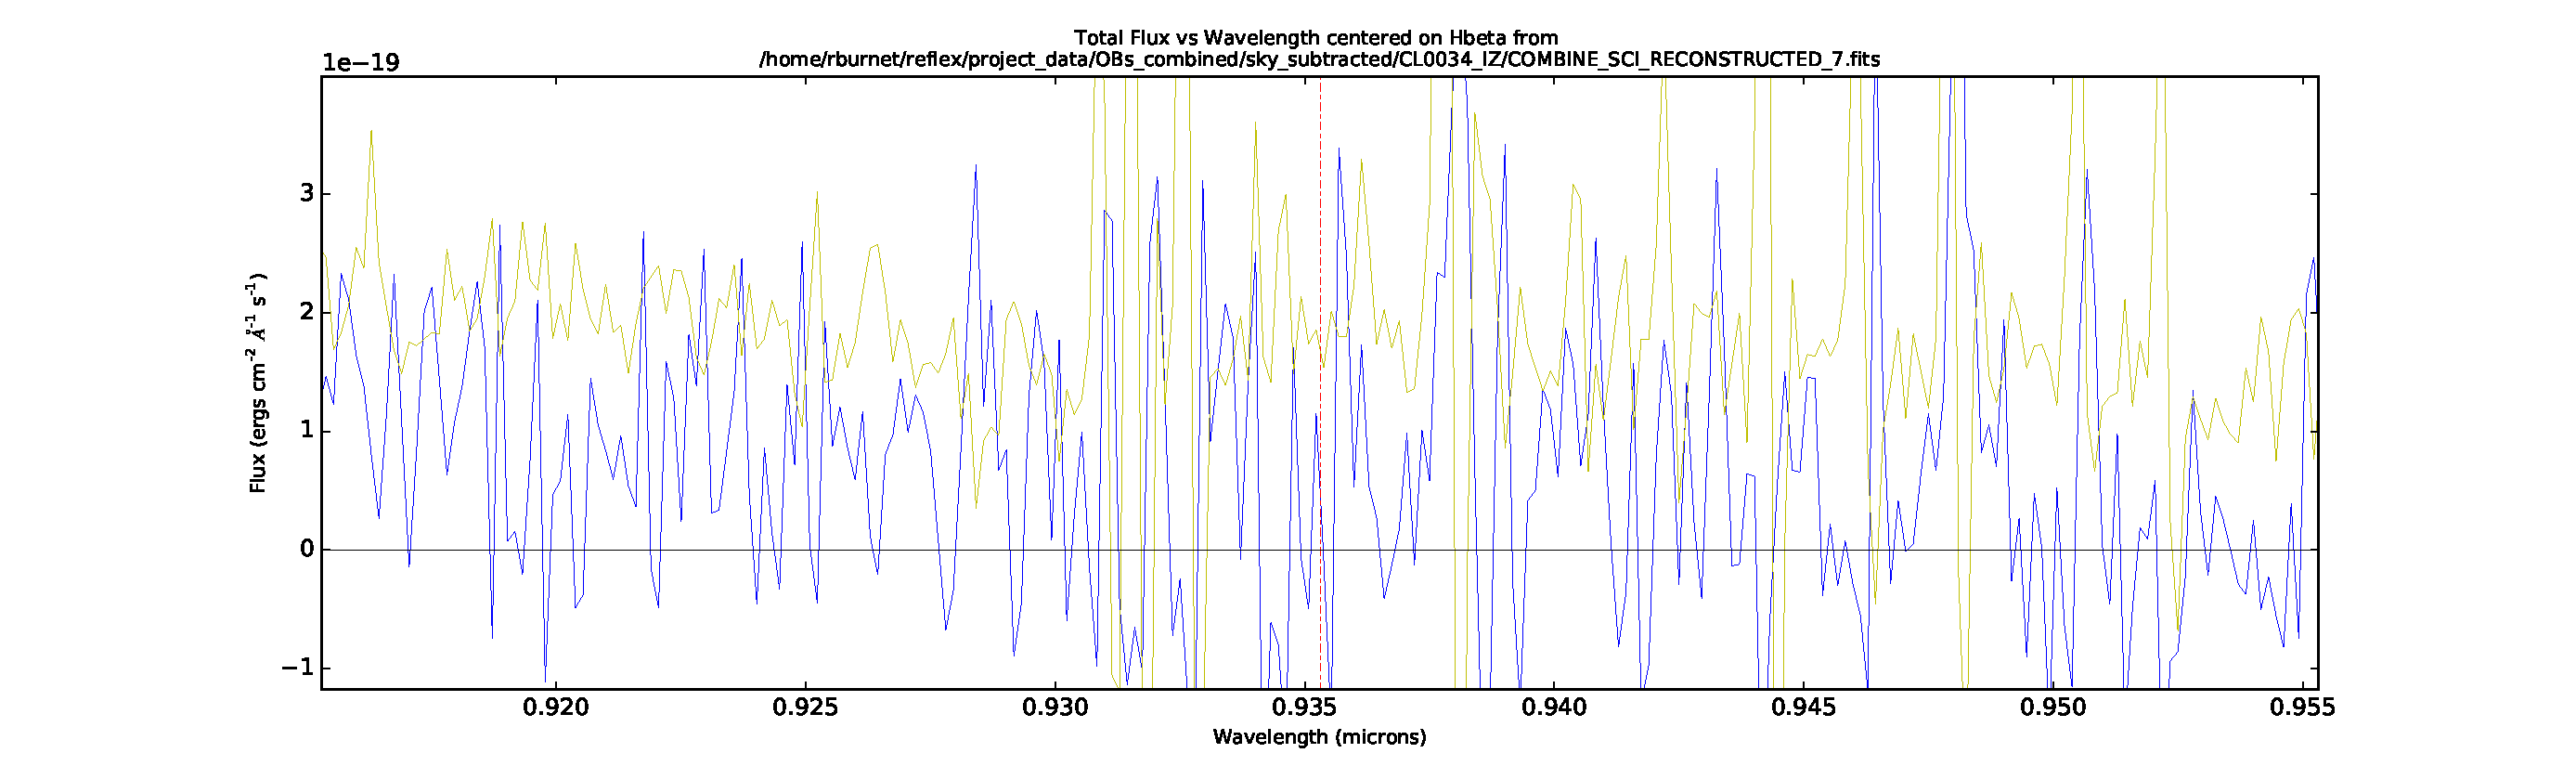
\includegraphics[scale=0.45]{../figures/CL0034_IZ/COMBINE_SCI_RECONSTRUCTED_7_OIII.pdf} \\
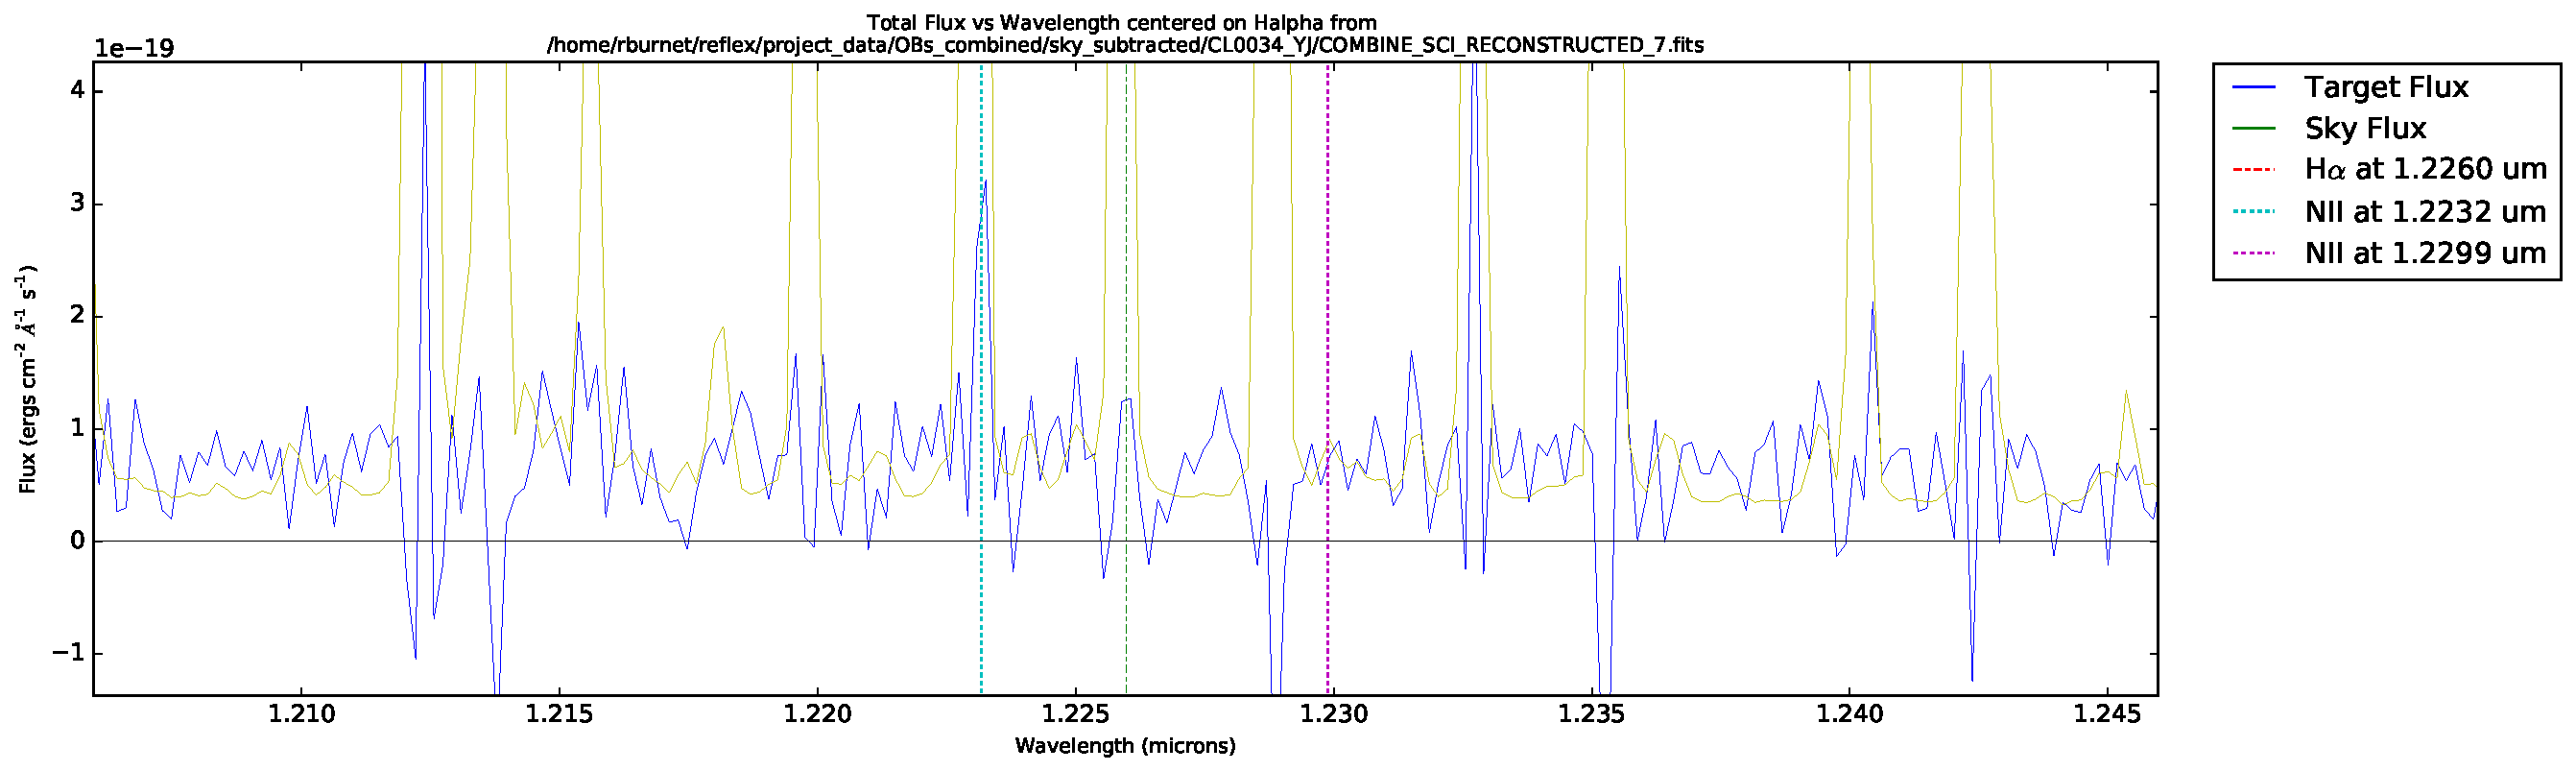
\includegraphics[scale=0.45]{../figures/CL0034_YJ/COMBINE_SCI_RECONSTRUCTED_7_Halpha.pdf}
\end{tabular}
\end{center}
\end{table}

\newpage

CL0034 Target 20, Arm 14 \\

\begin{table}[h!]
\begin{center}
\begin{tabular}{ >{\centering\arraybackslash}m{2.5in} >{\centering\arraybackslash}m{2.5in} >{\centering\arraybackslash}m{2.5in} >{\centering\arraybackslash}m{2.3in}}
HST Image & Collapsed YJ Image &  Collapsed IZ Image & \\
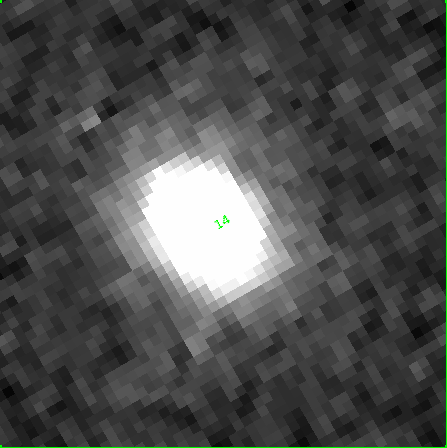
\includegraphics[scale=0.35]{/home/rburnet/S16work/diagnostic_of_objects/figures/HST_images/CL0034/CL0034-Target_20.png} 
&
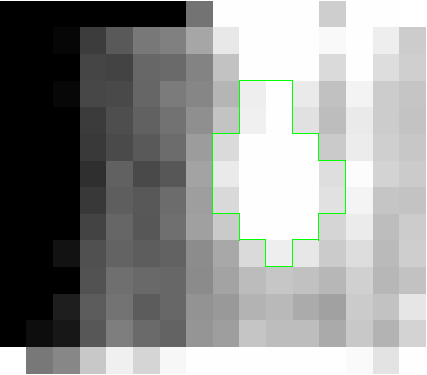
\includegraphics[scale=0.4]{/home/rburnet/S16work/diagnostic_of_objects/local_sky_subtraction/new_report/figures/CL0034-IZ-Target_20.png} 
&
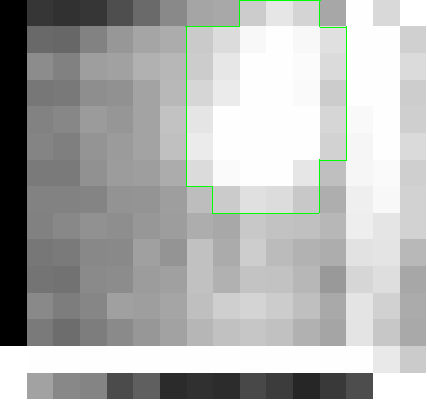
\includegraphics[scale=0.4]{/home/rburnet/S16work/diagnostic_of_objects/local_sky_subtraction/new_report/figures/CL0034-YJ-Target_20.png} 
\\
&
\begin{tabular}{ l l l }
M$_{\text{IZ, calculated}}$ & = &  20.33\\
M$_{\text{YJ, calculated}}$ & = &  20.07\\
M$_{\text{Z, expected}}$ & = & 21.73\\
F(H$\alpha) _{\text{expected}}$ & = & Unknown\\
F(H$\alpha) _{\text{expected, uncorrected}}$ & = & Unknown\\
\end{tabular} \\
\\
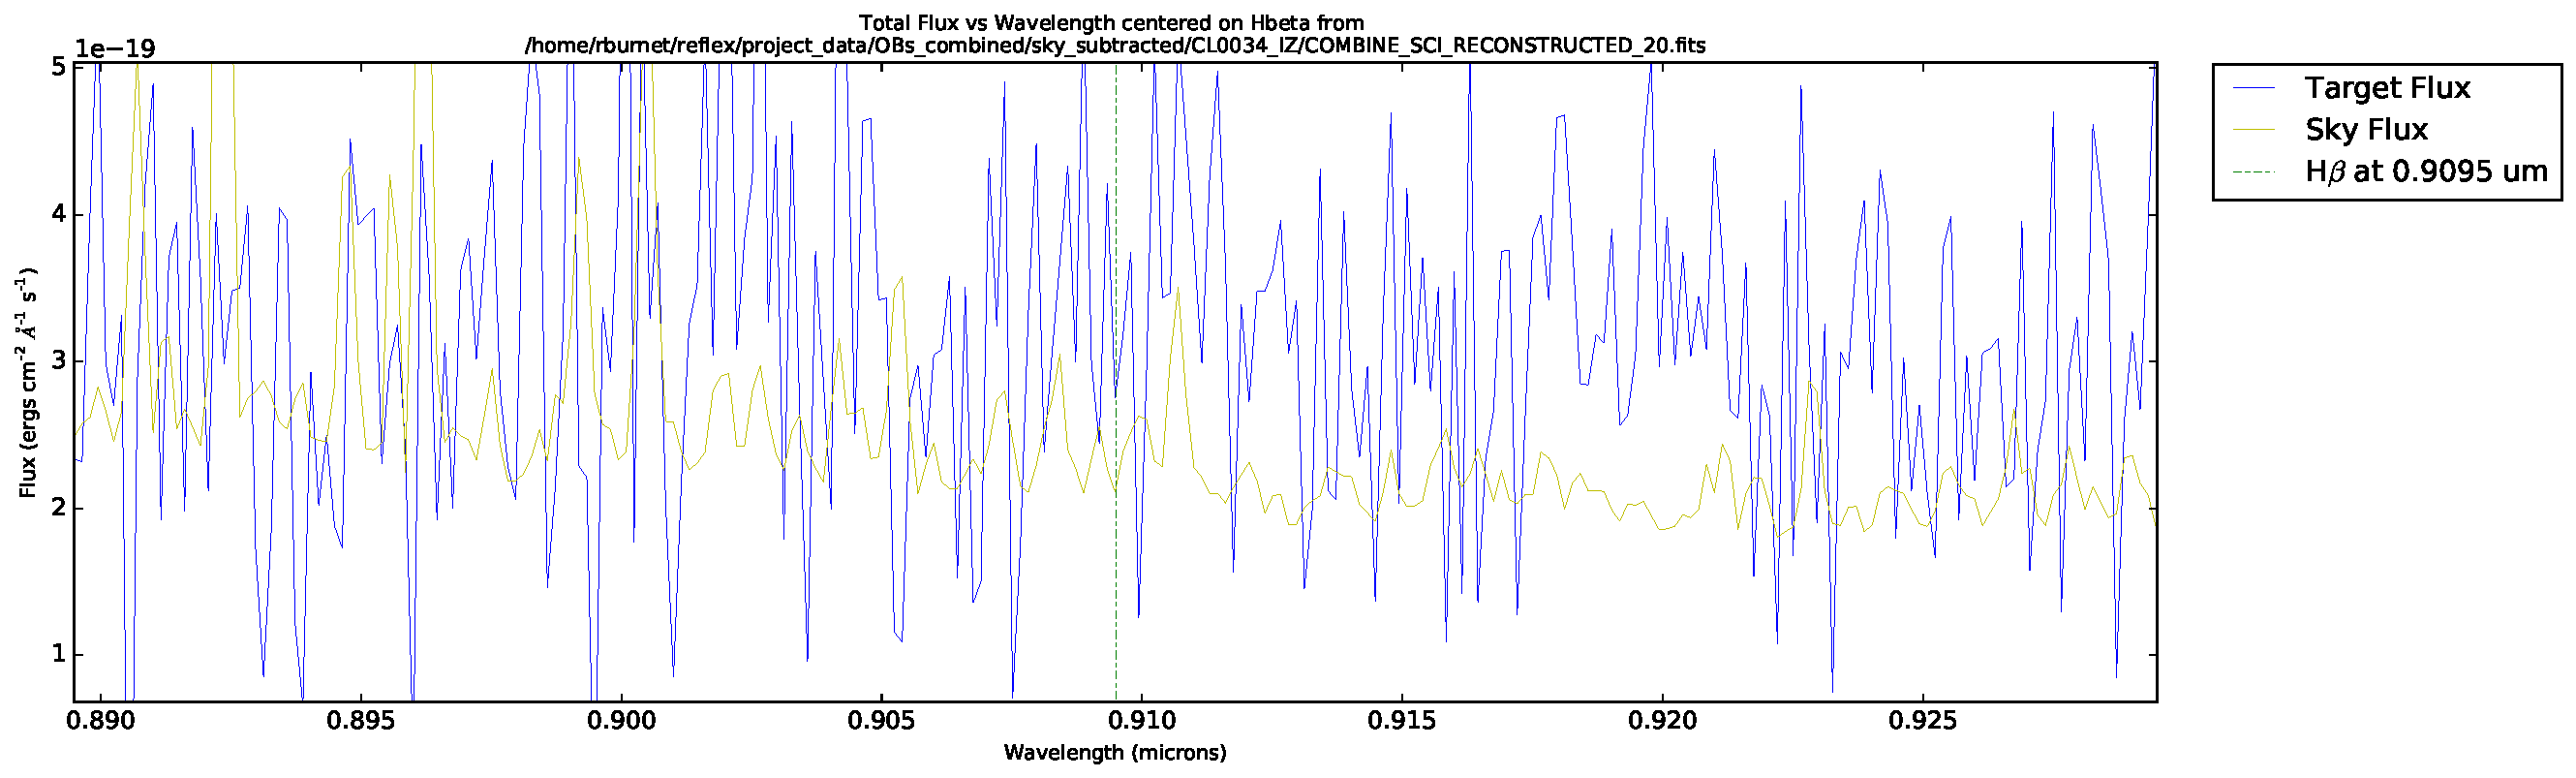
\includegraphics[scale=0.45]{../figures/CL0034_IZ/COMBINE_SCI_RECONSTRUCTED_20_Hbeta.pdf} \\
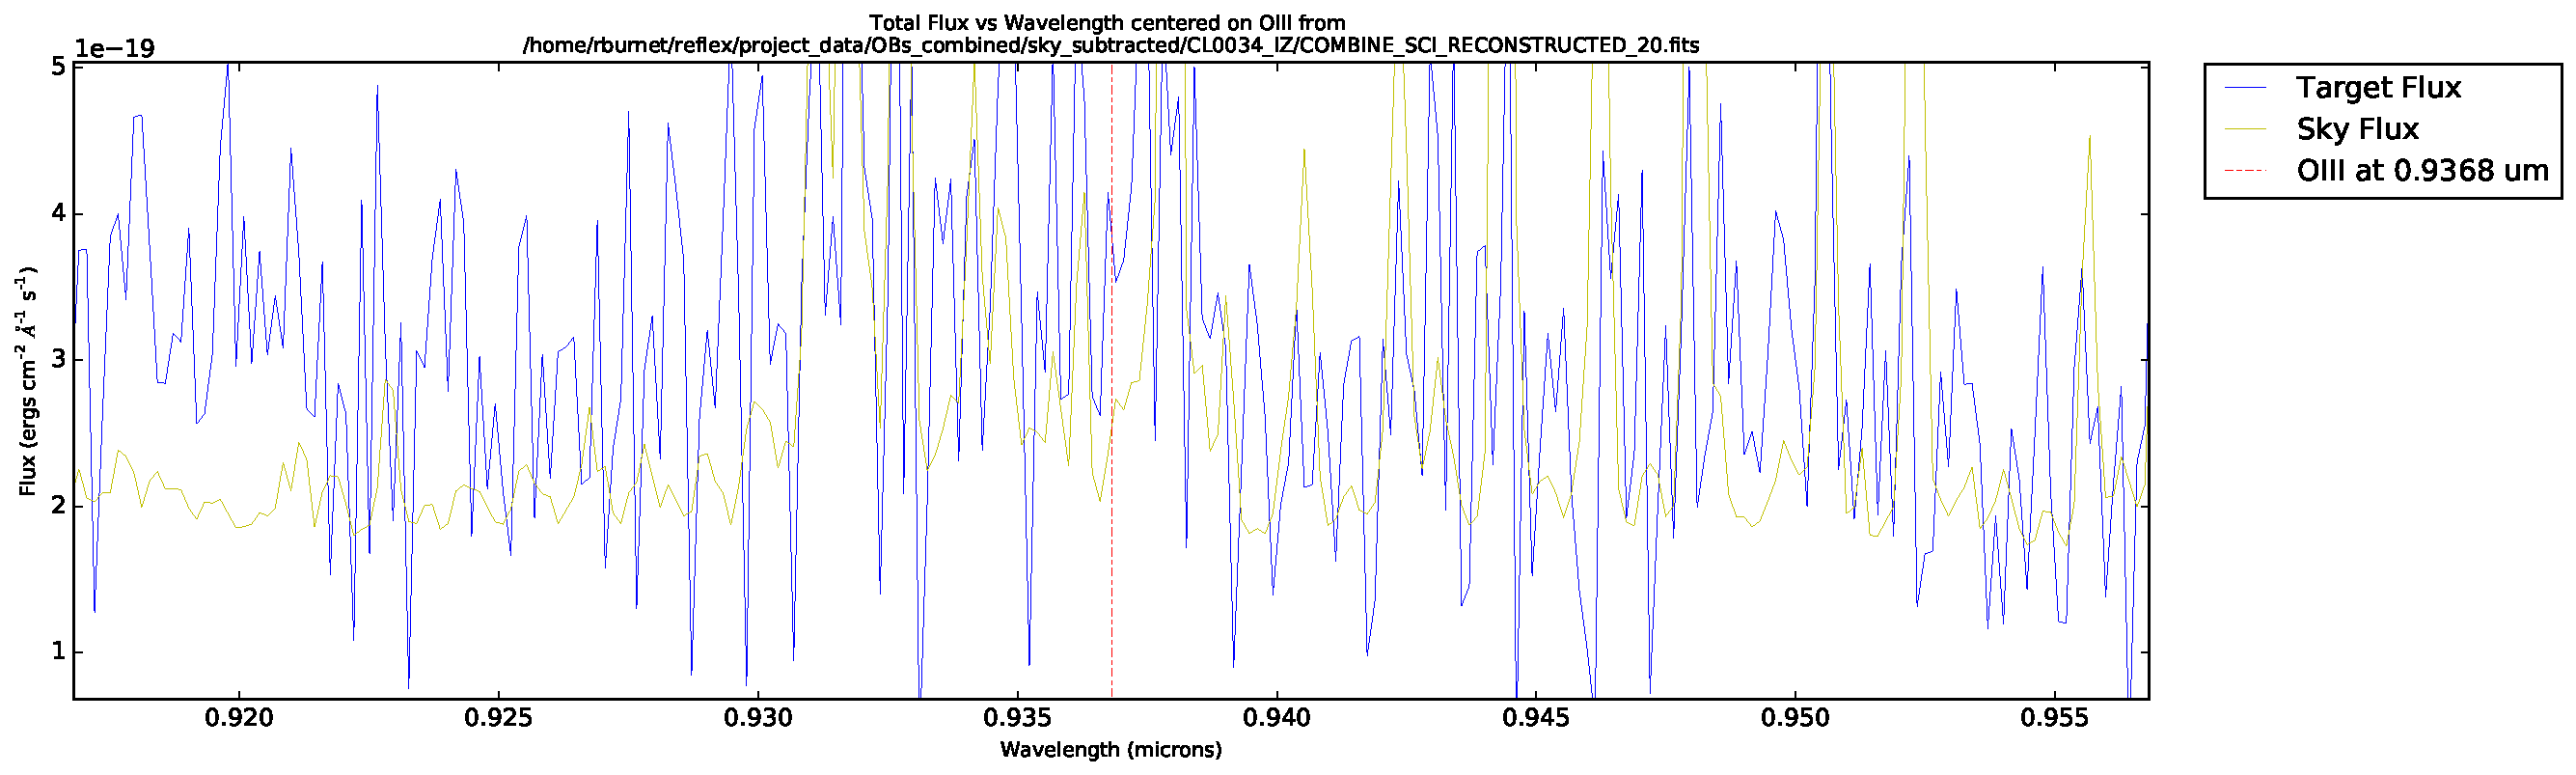
\includegraphics[scale=0.45]{../figures/CL0034_IZ/COMBINE_SCI_RECONSTRUCTED_20_OIII.pdf} \\
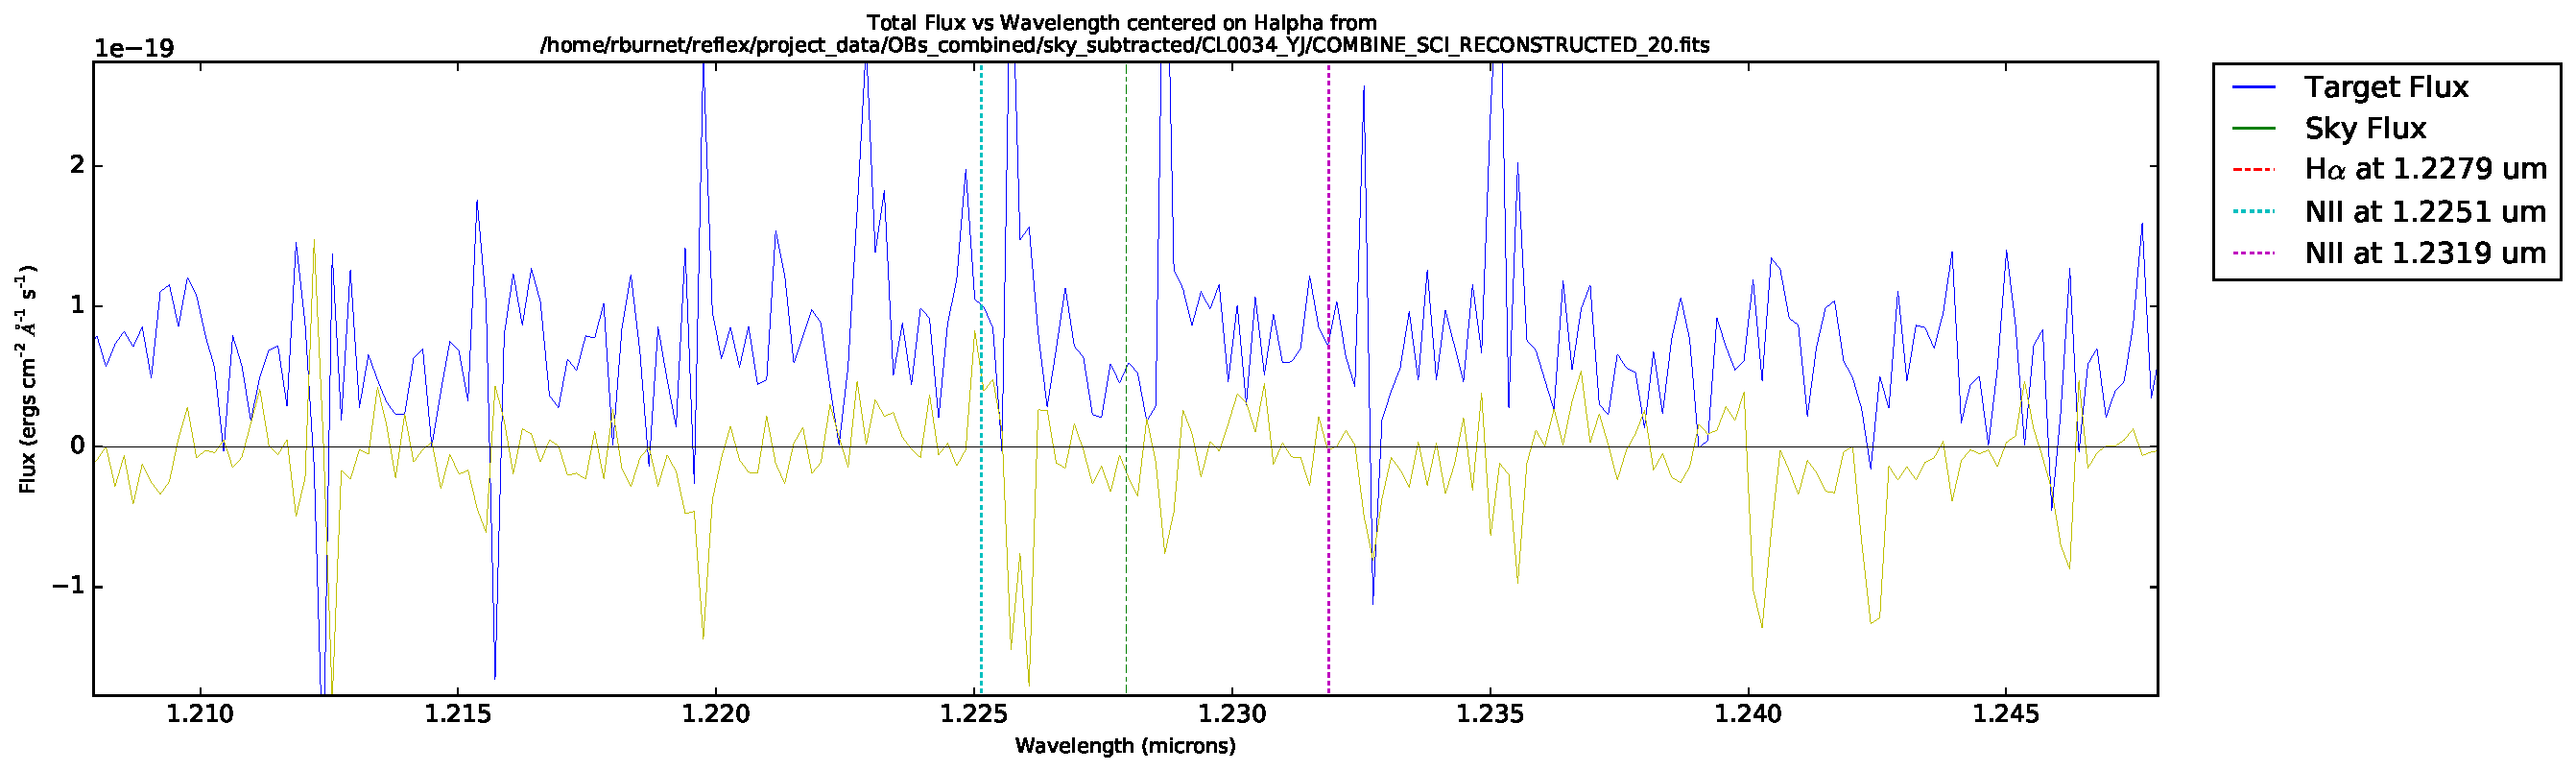
\includegraphics[scale=0.45]{../figures/CL0034_YJ/COMBINE_SCI_RECONSTRUCTED_20_Halpha.pdf}
\end{tabular}
\end{center}
\end{table}

\newpage
CL0034 Target 23, Arm 20 \\

\begin{table}[h!]
\begin{center}
\begin{tabular}{ >{\centering\arraybackslash}m{2.5in} >{\centering\arraybackslash}m{2.5in} >{\centering\arraybackslash}m{2.5in} >{\centering\arraybackslash}m{2.3in}}
HST Image & Collapsed YJ Image &  Collapsed IZ Image & \\
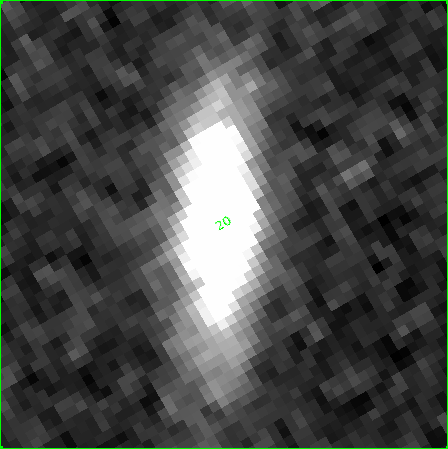
\includegraphics[scale=0.35]{/home/rburnet/S16work/diagnostic_of_objects/figures/HST_images/CL0034/CL0034-Target_23.png} 
&
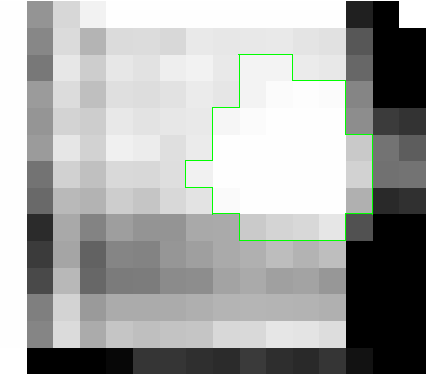
\includegraphics[scale=0.4]{/home/rburnet/S16work/diagnostic_of_objects/local_sky_subtraction/new_report/figures/CL0034-IZ-Target_23.png}
&
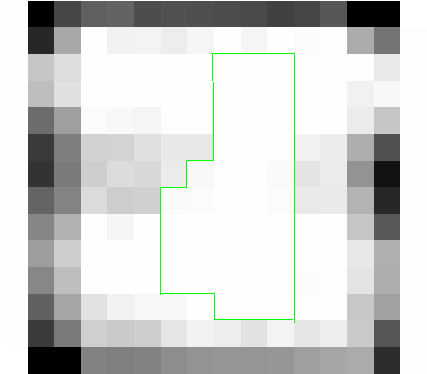
\includegraphics[scale=0.4]{/home/rburnet/S16work/diagnostic_of_objects/local_sky_subtraction/new_report/figures/CL0034-YJ-Target_23.png} 
\\
&
\begin{tabular}{ l l l }
M$_{\text{IZ, calculated}}$ & = &  21.00\\
M$_{\text{YJ, calculated}}$ & = &  21.44\\
M$_{\text{Z, expected}}$ & = & 22.08\\
F(H$\alpha) _{\text{expected}}$ & = & Unknown\\
F(H$\alpha) _{\text{expected, uncorrected}}$ & = & Unknown\\
\end{tabular} \\
\\
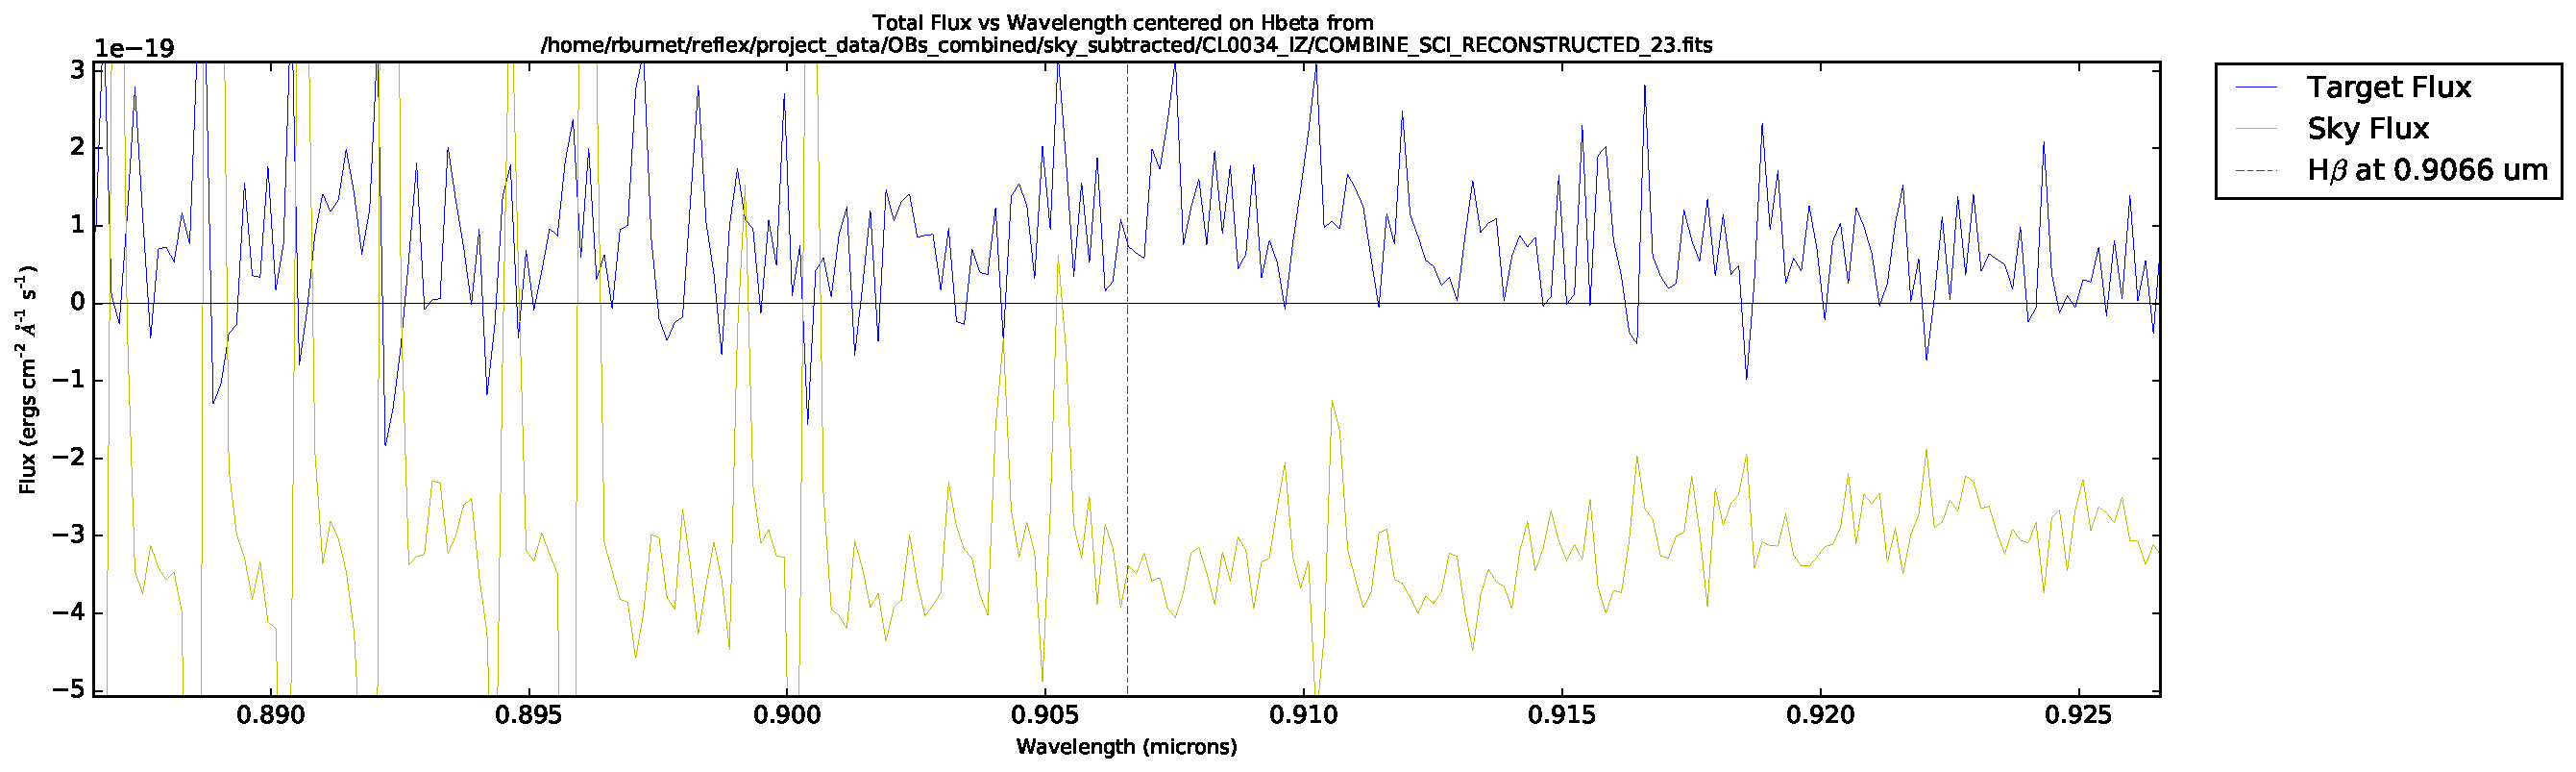
\includegraphics[scale=0.45]{../figures/CL0034_IZ/COMBINE_SCI_RECONSTRUCTED_23_Hbeta.pdf} \\
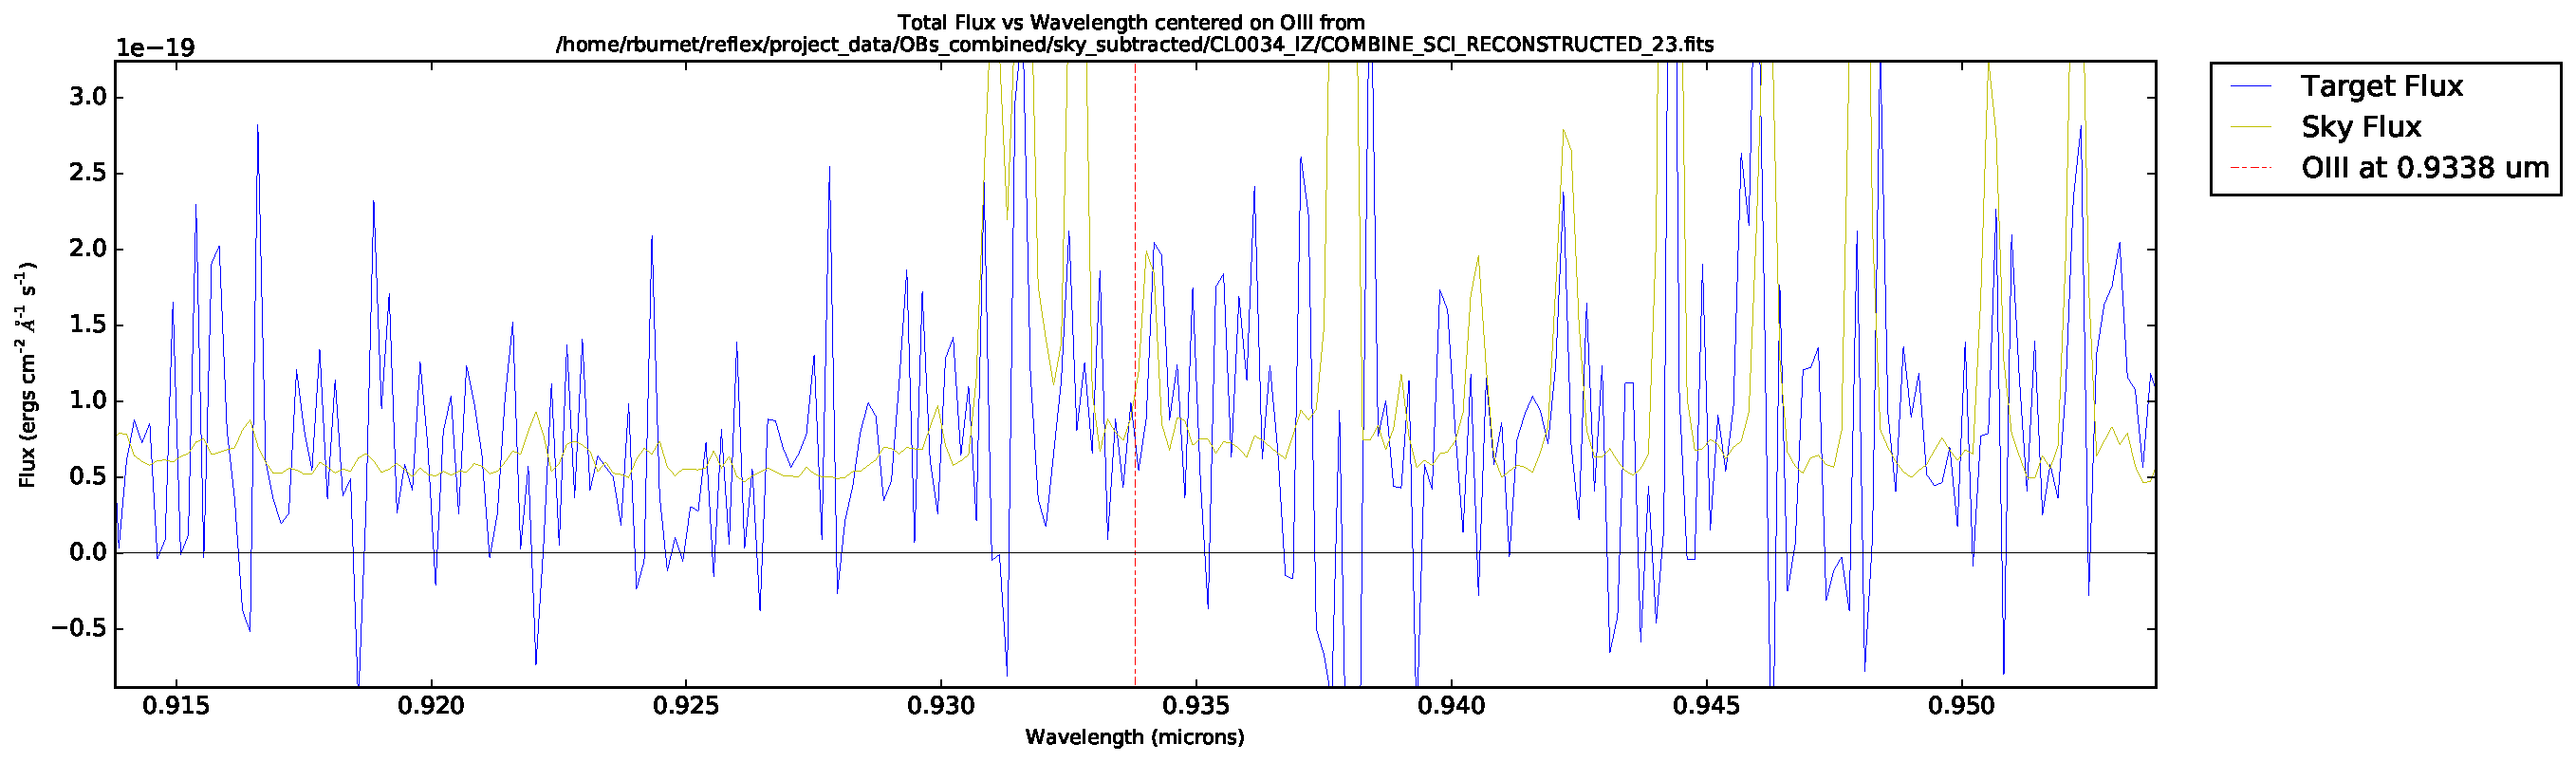
\includegraphics[scale=0.45]{../figures/CL0034_IZ/COMBINE_SCI_RECONSTRUCTED_23_OIII.pdf} \\
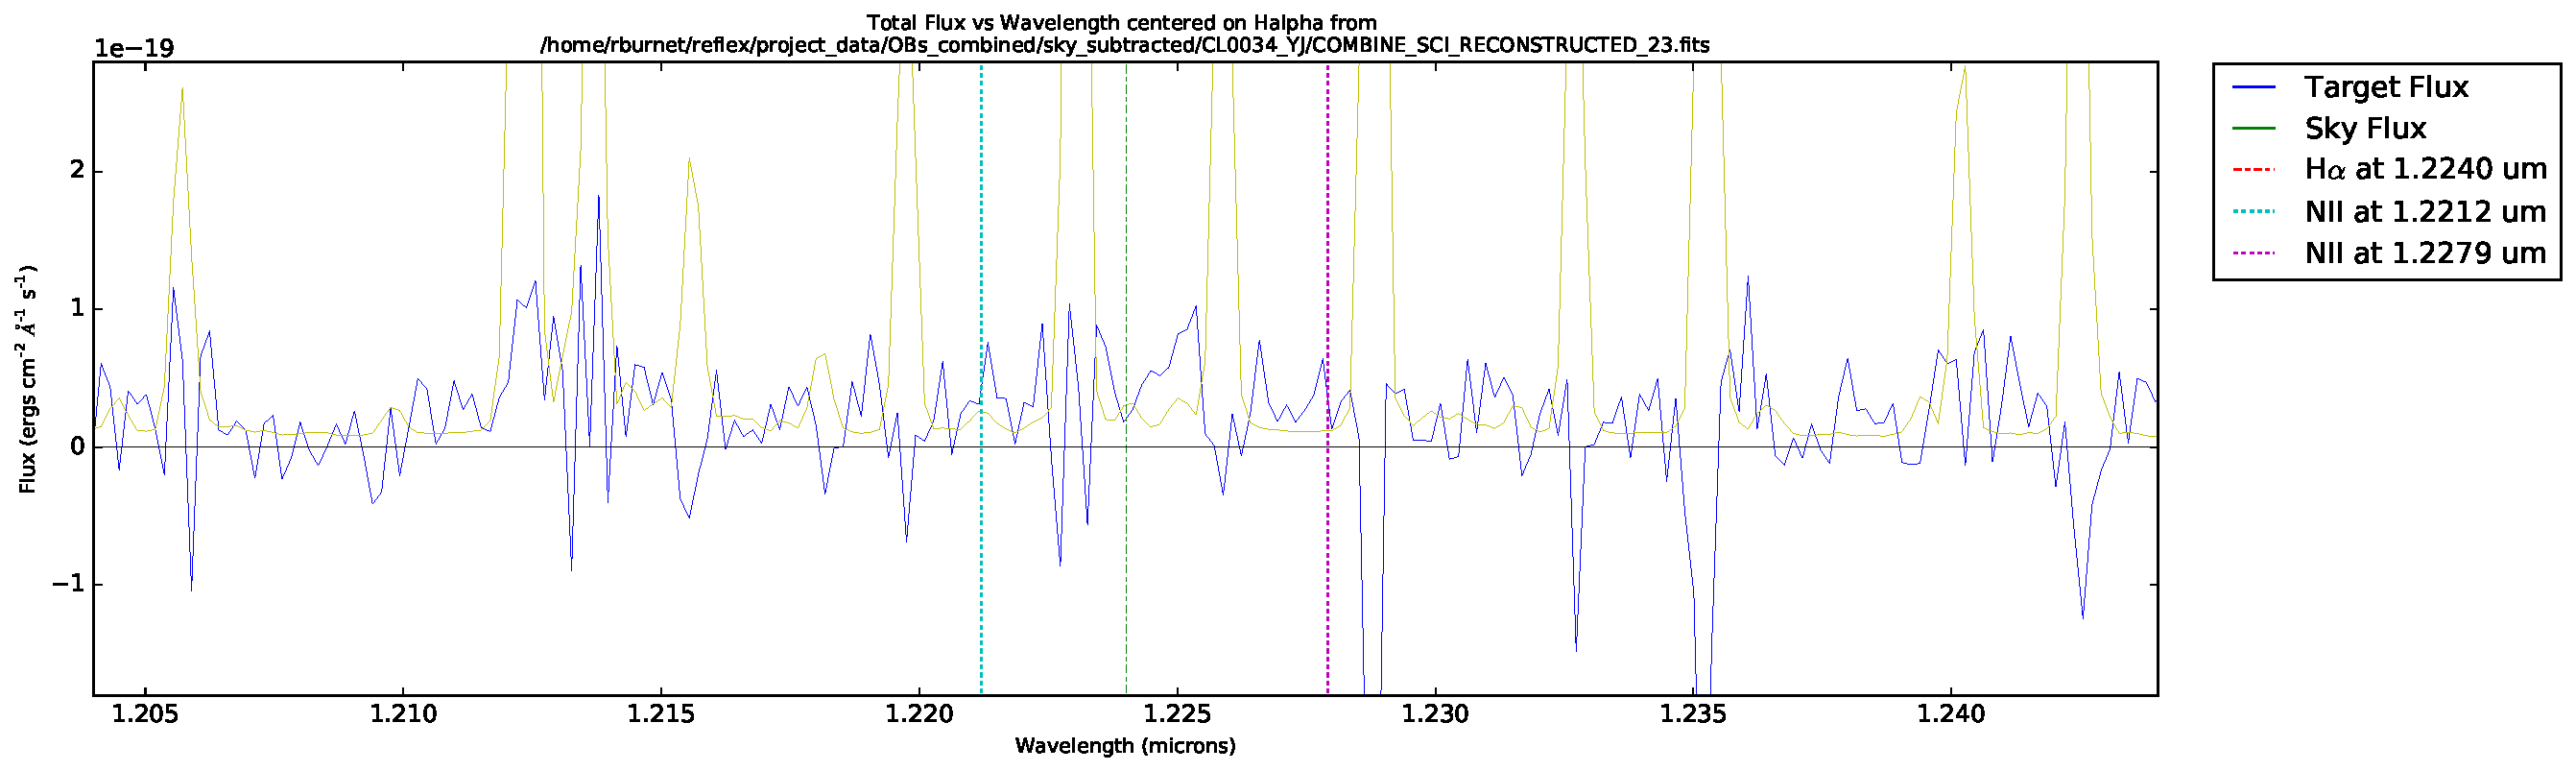
\includegraphics[scale=0.45]{../figures/CL0034_YJ/COMBINE_SCI_RECONSTRUCTED_23_Halpha.pdf}
\end{tabular}
\end{center}
\end{table}

\newpage

CL0034 Target 22, Arm 11 \\

\begin{table}[h!]
\begin{center}
\begin{tabular}{ >{\centering\arraybackslash}m{2.5in} >{\centering\arraybackslash}m{2.5in} >{\centering\arraybackslash}m{2.5in} >{\centering\arraybackslash}m{2.3in}}
HST Image & Collapsed YJ Image &  Collapsed IZ Image & \\
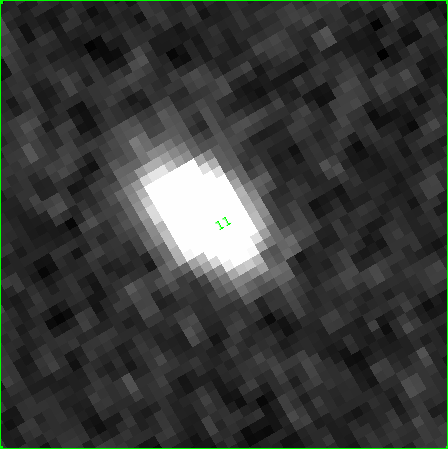
\includegraphics[scale=0.35]{/home/rburnet/S16work/diagnostic_of_objects/figures/HST_images/CL0034/CL0034-Target_22.png} 
&
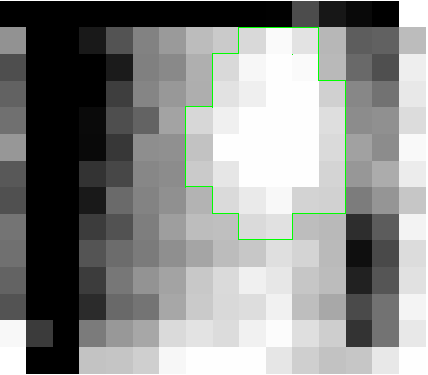
\includegraphics[scale=0.4]{/home/rburnet/S16work/diagnostic_of_objects/local_sky_subtraction/new_report/figures/CL0034-IZ-Target_22.png}
&

\includegraphics[scale=0.4]{/home/rburnet/S16work/diagnostic_of_objects/local_sky_subtraction/new_report/figures/CL0034-YJ-Target_22.png} 
\\
&
\begin{tabular}{ l l l }
M$_{\text{IZ, calculated}}$ & = &  21.22\\
M$_{\text{YJ, calculated}}$ & = &  21.02\\
M$_{\text{Z, expected}}$ & = & 22.27\\
F(H$\alpha) _{\text{expected}}$ & = & Unknown\\
F(H$\alpha) _{\text{expected, uncorrected}}$ & = & Unknown\\
\end{tabular} \\
\\
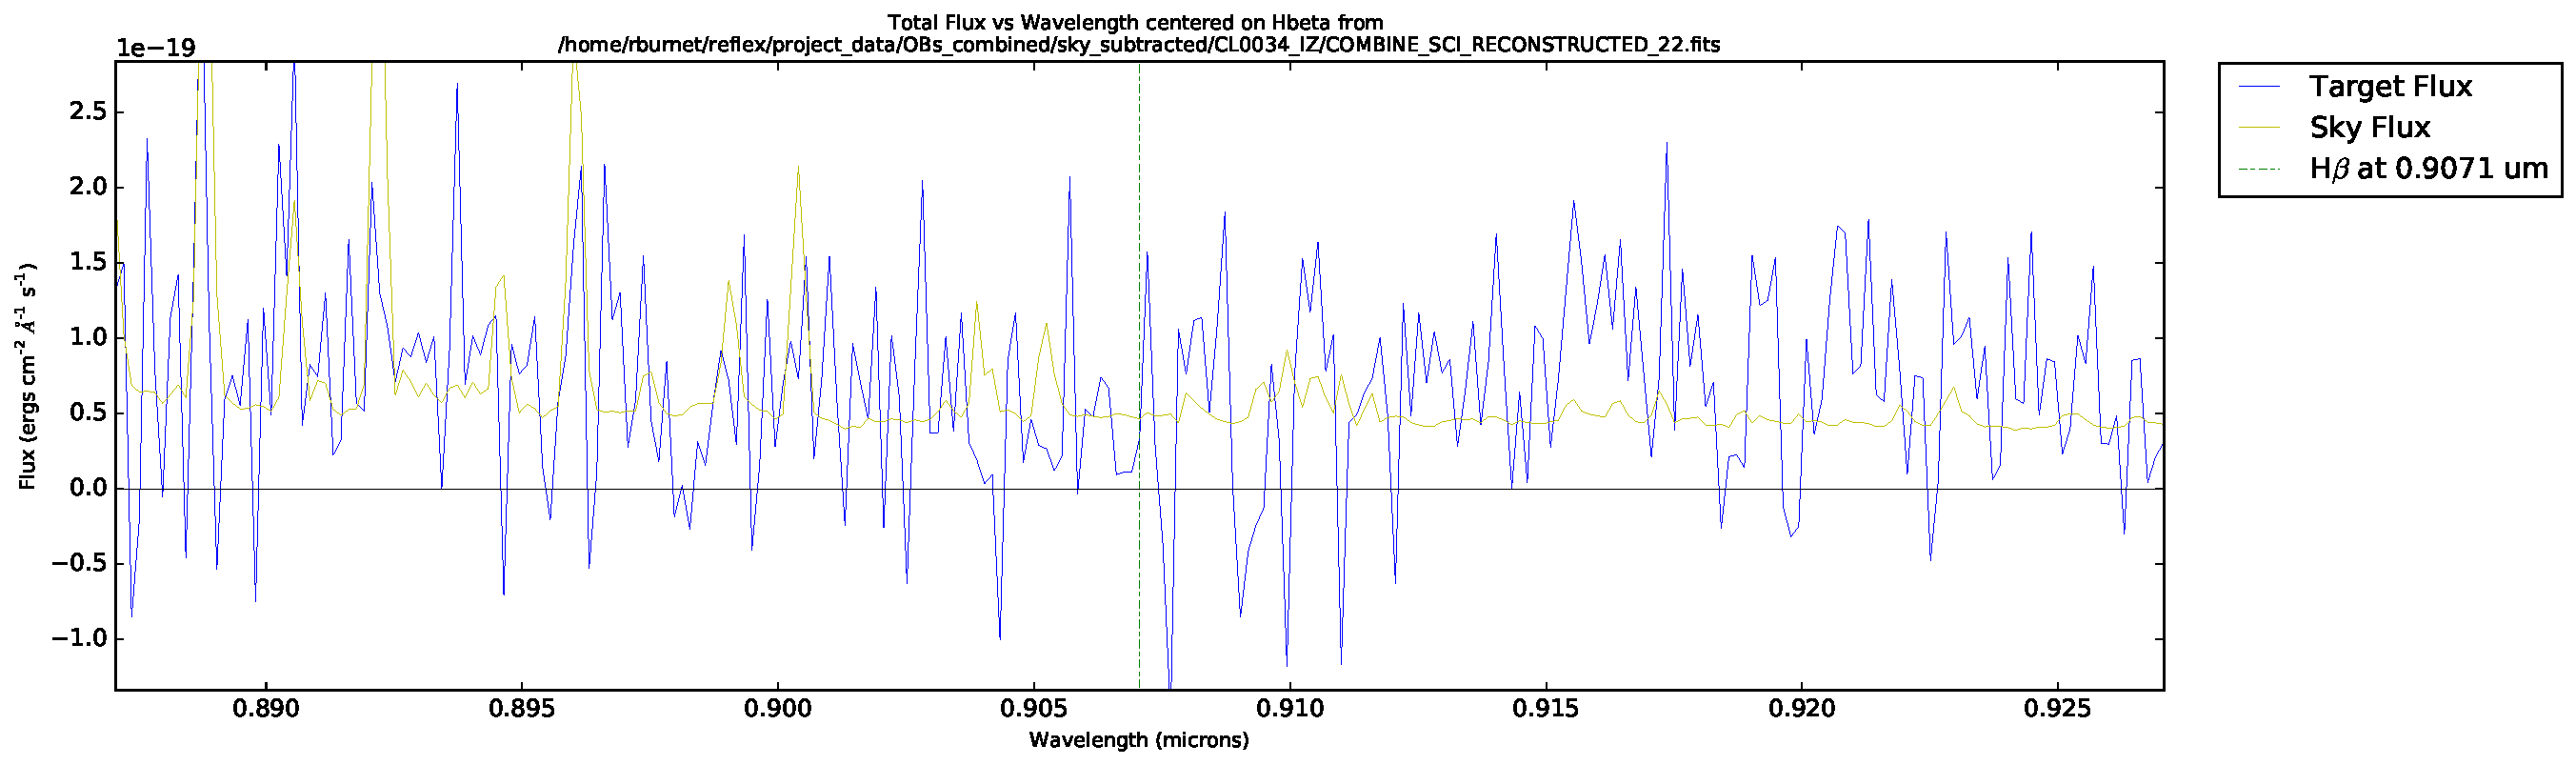
\includegraphics[scale=0.45]{../figures/CL0034_IZ/COMBINE_SCI_RECONSTRUCTED_22_Hbeta.pdf} \\
\includegraphics[scale=0.45]{../figures/CL0034_IZ/COMBINE_SCI_RECONSTRUCTED_22_OIII.pdf} \\
\includegraphics[scale=0.45]{../figures/CL0034_YJ/COMBINE_SCI_RECONSTRUCTED_22_Halpha.pdf}
\end{tabular}
\end{center}
\end{table}

\newpage
CL0034 Target 6, Arm 24 \\

\begin{table}[h!]
\begin{center}
\begin{tabular}{ >{\centering\arraybackslash}m{2.5in} >{\centering\arraybackslash}m{2.5in} >{\centering\arraybackslash}m{2.5in} >{\centering\arraybackslash}m{2.3in}}
HST Image & Collapsed YJ Image &  Collapsed IZ Image & \\
\includegraphics[scale=0.35]{/home/rburnet/S16work/diagnostic_of_objects/figures/HST_images/CL0034/CL0034-Target_6.png} 
&
\includegraphics[scale=0.4]{/home/rburnet/S16work/diagnostic_of_objects/local_sky_subtraction/new_report/figures/CL0034-IZ-Target_6.png} 
&
\includegraphics[scale=0.4]{/home/rburnet/S16work/diagnostic_of_objects/local_sky_subtraction/new_report/figures/CL0034-YJ-Target_6.png}
\\ 
&
\begin{tabular}{ l l l }
M$_{\text{IZ, calculated}}$ & = &  22.52\\
M$_{\text{YJ, calculated}}$ & = &  21.93\\
M$_{\text{Z, expected}}$ & = & 22.37\\
F(H$\alpha) _{\text{expected}}$ & = & 2.489e-16\\
F(H$\alpha) _{\text{expected, uncorrected}}$ & = & 6.364e-16\\
\end{tabular} \\
\\
\includegraphics[scale=0.45]{../figures/CL0034_IZ/COMBINE_SCI_RECONSTRUCTED_6_Hbeta.pdf} \\
\includegraphics[scale=0.45]{../figures/CL0034_IZ/COMBINE_SCI_RECONSTRUCTED_6_OIII.pdf} \\
\includegraphics[scale=0.45]{../figures/CL0034_YJ/COMBINE_SCI_RECONSTRUCTED_6_Halpha.pdf}
\end{tabular}
\end{center}
\end{table}

\newpage

CL0034 Target 26, Arm 9 \\

\begin{table}[h!]
\begin{center}
\begin{tabular}{ >{\centering\arraybackslash}m{2.5in} >{\centering\arraybackslash}m{2.5in} >{\centering\arraybackslash}m{2.5in} >{\centering\arraybackslash}m{2.3in}}
HST Image & Collapsed YJ Image &  Collapsed IZ Image & \\
\includegraphics[scale=0.35]{/home/rburnet/S16work/diagnostic_of_objects/figures/HST_images/CL0034/CL0034-Target_26.png} 
&
\includegraphics[scale=0.4]{/home/rburnet/S16work/diagnostic_of_objects/local_sky_subtraction/new_report/figures/CL0034-IZ-Target_26.png} 
&
\includegraphics[scale=0.4]{/home/rburnet/S16work/diagnostic_of_objects/local_sky_subtraction/new_report/figures/CL0034-YJ-Target_26.png} 
\\
&
\begin{tabular}{ l l l }
M$_{\text{IZ, calculated}}$ & = &  19.66\\
M$_{\text{YJ, calculated}}$ & = &  20.73\\
M$_{\text{Z, expected}}$ & = & 22.40\\
F(H$\alpha) _{\text{expected}}$ & = & Unknown\\
F(H$\alpha) _{\text{expected, uncorrected}}$ & = & Unknown\\
\end{tabular} \\
\\
\includegraphics[scale=0.45]{../figures/CL0034_IZ/COMBINE_SCI_RECONSTRUCTED_26_Hbeta.pdf} \\
\includegraphics[scale=0.45]{../figures/CL0034_IZ/COMBINE_SCI_RECONSTRUCTED_26_OIII.pdf} \\
\includegraphics[scale=0.45]{../figures/CL0034_YJ/COMBINE_SCI_RECONSTRUCTED_26_Halpha.pdf}
\end{tabular}
\end{center}
\end{table}

\newpage
CL0034 Target 14, Arm 8 \\

\begin{table}[h!]
\begin{center}
\begin{tabular}{ >{\centering\arraybackslash}m{2.5in} >{\centering\arraybackslash}m{2.5in} >{\centering\arraybackslash}m{2.5in} >{\centering\arraybackslash}m{2.3in}}
HST Image & Collapsed YJ Image &  Collapsed IZ Image & \\
\includegraphics[scale=0.35]{/home/rburnet/S16work/diagnostic_of_objects/figures/HST_images/CL0034/CL0034-Target_14.png} 
& 
\includegraphics[scale=0.4]{/home/rburnet/S16work/diagnostic_of_objects/local_sky_subtraction/new_report/figures/CL0034-IZ-Target_14.png} 
&
\includegraphics[scale=0.4]{/home/rburnet/S16work/diagnostic_of_objects/local_sky_subtraction/new_report/figures/CL0034-YJ-Target_14.png} 
\\
&
\begin{tabular}{ l l l }
M$_{\text{IZ, calculated}}$ & = &  22.28\\
M$_{\text{YJ, calculated}}$ & = &  21.64\\
M$_{\text{Z, expected}}$ & = & 22.49\\
F(H$\alpha) _{\text{expected}}$ & = & 2.337e-16\\
F(H$\alpha) _{\text{expected, uncorrected}}$ & = & 5.260e-16\\
\end{tabular} \\
\\
\includegraphics[scale=0.45]{../figures/CL0034_IZ/COMBINE_SCI_RECONSTRUCTED_14_Hbeta.pdf} \\
\includegraphics[scale=0.45]{../figures/CL0034_IZ/COMBINE_SCI_RECONSTRUCTED_14_OIII.pdf} \\
\includegraphics[scale=0.45]{../figures/CL0034_YJ/COMBINE_SCI_RECONSTRUCTED_14_Halpha.pdf}
\end{tabular}
\end{center}
\end{table}

\newpage 

CL0034 Target 16, Arm 19 \\

\begin{table}[h!]
\begin{center}
\begin{tabular}{ >{\centering\arraybackslash}m{2.5in} >{\centering\arraybackslash}m{2.5in} >{\centering\arraybackslash}m{2.5in} >{\centering\arraybackslash}m{2.3in}}
HST Image & Collapsed YJ Image &  Collapsed IZ Image & \\
\includegraphics[scale=0.35]{/home/rburnet/S16work/diagnostic_of_objects/figures/HST_images/CL0034/CL0034-Target_16.png} 
& 
\includegraphics[scale=0.4]{/home/rburnet/S16work/diagnostic_of_objects/local_sky_subtraction/new_report/figures/CL0034-IZ-Target_16.png} 
&
\includegraphics[scale=0.4]{/home/rburnet/S16work/diagnostic_of_objects/local_sky_subtraction/new_report/figures/CL0034-YJ-Target_16.png} 
\\
&
\begin{tabular}{ l l l }
M$_{\text{IZ, calculated}}$ & = & 20.01\\
M$_{\text{YJ, calculated}}$ & = & 20.17\\
M$_{\text{Z, expected}}$ & = & 22.50\\
F(H$\alpha) _{\text{expected}}$ & = & 2.629e-16\\
F(H$\alpha) _{\text{expected, uncorrected}}$ & = & 4.994e-16\\
\end{tabular} \\
\\
\includegraphics[scale=0.45]{../figures/CL0034_IZ/COMBINE_SCI_RECONSTRUCTED_16_Hbeta.pdf} \\
\includegraphics[scale=0.45]{../figures/CL0034_IZ/COMBINE_SCI_RECONSTRUCTED_16_OIII.pdf} \\
\includegraphics[scale=0.45]{../figures/CL0034_YJ/COMBINE_SCI_RECONSTRUCTED_16_Halpha.pdf}
\end{tabular}
\end{center}
\end{table}

\newpage
CL0034 Target 21, Arm 12 \\

\begin{table}[h!]
\begin{center}
\begin{tabular}{ >{\centering\arraybackslash}m{2.5in} >{\centering\arraybackslash}m{2.5in} >{\centering\arraybackslash}m{2.5in} >{\centering\arraybackslash}m{2.3in}}
HST Image & Collapsed YJ Image &  Collapsed IZ Image & \\
\includegraphics[scale=0.35]{/home/rburnet/S16work/diagnostic_of_objects/figures/HST_images/CL0034/CL0034-Target_21.png} 
& 
\includegraphics[scale=0.4]{/home/rburnet/S16work/diagnostic_of_objects/local_sky_subtraction/new_report/figures/CL0034-IZ-Target_21.png} 
&
\includegraphics[scale=0.4]{/home/rburnet/S16work/diagnostic_of_objects/local_sky_subtraction/new_report/figures/CL0034-YJ-Target_21.png} 
\\
&
\begin{tabular}{ l l l }
M$_{\text{IZ, calculated}}$ & = & 21.11\\
M$_{\text{YJ, calculated}}$ & = & 21.93\\
M$_{\text{Z, expected}}$ & = & 22.91\\
F(H$\alpha) _{\text{expected}}$ & = & Unknown\\
F(H$\alpha) _{\text{expected, uncorrected}}$ & = & Unknown\\
\end{tabular} \\
\\
\includegraphics[scale=0.45]{../figures/CL0034_IZ/COMBINE_SCI_RECONSTRUCTED_21_Hbeta.pdf} \\
\includegraphics[scale=0.45]{../figures/CL0034_IZ/COMBINE_SCI_RECONSTRUCTED_21_OIII.pdf} \\
\includegraphics[scale=0.45]{../figures/CL0034_YJ/COMBINE_SCI_RECONSTRUCTED_21_Halpha.pdf}
\end{tabular}
\end{center}
\end{table} 

\end{document}
